\documentclass[12pt,a4paper,twoside]{report}
\usepackage[left=3cm,right=3cm,top=3cm,bottom=3cm,headsep=0.25in, voffset= 0.0in]{geometry}
\usepackage{pagenote}

%algo packages
\usepackage{algorithm}
\usepackage{algorithmic}

%color packages
\usepackage{xcolor}
\colorlet{shadecolor}{orange!15}
\usepackage{color,soul}
\usepackage{soulutf8}
\definecolor{bordeau}{rgb}{0.3515625,0,0.234375}

% position of figure
\usepackage[absolute,overlay]{textpos}

%graphic packages
\usepackage{graphicx}
\graphicspath{ {figures/} }
\usepackage{wrapfig}
\usepackage{float} 
\usepackage{tikz}
\usepackage{pgfplots}
\usepackage{pgfplotstable}

% table packages
\usepackage{array}
\usepackage{multirow,booktabs}
\usepackage{multicol}
\usepackage{tabularx}

% font package
\usepackage[utf8]{inputenc}	% Para caracteres en español
\usepackage{textcomp}
%\usepackage{times}
%\usepackage{lmodern}
\usepackage{mathptmx}

% equation packages
\usepackage{amsmath,amsthm,amsfonts,amssymb,amscd}
\usepackage{mathrsfs}

% header, footer packages
\pagestyle{headings}

% page package
\usepackage{enumitem}
\usepackage{fancyhdr}
\fancyhf{}
\fancyhead[LE]{\nouppercase{\leftmark}}
\fancyhead[RO]{\nouppercase{\rightmark}}
\fancyfoot[LE,RO]{\thepage}
\pagestyle{fancy}
\usepackage{afterpage}

% space package
\usepackage{setspace}
\usepackage{calc}
\usepackage{color,soul}
\usepackage{cancel}
\usepackage{listings}
\usepackage{titlesec}
\titlespacing*{\section}
{0pt}{1.0ex}{1.0ex}
\titlespacing*{\chapter}
{0pt}{1.5ex}{2.0ex}
\titlespacing*{\subsection}
{0pt}{1.0ex}{1.0ex}

\setlength{\belowdisplayskip}{8pt} \setlength{\belowdisplayshortskip}{8pt}
\setlength{\abovedisplayskip}{8pt} \setlength{\abovedisplayshortskip}{8pt}
\setlist{nosep}
\setlength{\parskip}{0.1cm}
\setlength{\parindent}{1em}
%\renewcommand{\baselinestretch}{0.5}

% theorem commands
\theoremstyle{definition}
\newtheorem{lemma}{Lemma}[section]
\newtheorem{theorem}{Theorem}[section]
\newtheorem{proposition}{Proposition}[section]
\newtheorem{definition}{Definition}[section]

% verbatim env
\usepackage{fancyvrb}
\usepackage{spverbatim}

% reference
\usepackage[hidelinks]{hyperref}

% abbreviation package
\usepackage[nottoc]{tocbibind}
\usepackage[intoc]{nomencl}
\makenomenclature
\setlength{\nomlabelwidth}{2cm}
\setlength{\nomitemsep}{-1.5\parsep}
\renewcommand{\nomname}{List of Abbreviations}
\setcounter{tocdepth}{2}

\def\altand{\&}
%%\nomenclature[⟨prefix⟩]{⟨symbol⟩}{⟨description⟩}: the prefix is used to sort the abbreviations in the printing list.

%bibliography
\usepackage{natbib}
\setlength{\bibsep}{10.0pt}

% new command
\def\-{\raisebox{.75pt}{-}}
\DeclareMathOperator*{\argmax}{argmax}
\usepackage[draft]{todo}
\newcommand{\fyTodo}[1]{\Todo[FY:]{\textcolor{orange}{#1}}}
\newcommand{\fyTodostar}[1]{\Todo*[FY:]{\textcolor{orange}{#1}}}
\newcommand{\fyDone}[1]{\done[FY]\Todo[FY:]{\textcolor{orange}{#1}}}
\newcommand{\fyDonestar}[1]{\done[FY]\Todo[FY:]{\textcolor{orange}{#1}}}
\usepackage{titlesec}
\pgfkeys{
    /tr/rowfilter/.style 2 args={
        /pgfplots/x filter/.append code={
            \edef\arga{\thisrow{#1}}
            \edef\argb{#2}
            \ifx\arga\argb
            \else
                \def\pgfmathresult{}
            \fi
        }
    }
}
\newcommand{\system}[1]{\texttt{{#1}}}

%%%%%%%%%%%%%%%%%%%%%%%%%%%%%%%%%%%%%%%%%%%%%%%%

\newcommand\blankpage{%
    \null
    \thispagestyle{empty}%
    \addtocounter{page}{-1}%
    \newpage}

% Thesis title
\newcommand{\PhDTitle}{Multi-domain neural machine translation} 

% Name
\newcommand{\PhDname}{Minh-Quang PHAM}

%%%%%%%%%%%%%%%%%%%%%%%%%%%%%%%%%%%%%%%%%%%%%%%%


\begin{document}

	\doublespacing	

    %%%%%%%%%%%%%%%%%%%%%%%%%%%%%%%%%%%%%%%%%%%%%%%%%%%%%%%%%%%%%%%%%%%%%%%%%%%%%%%%%%%%%%%%%%%%%%%%%%%%%%%%%%%%%%%%%%%%%%%%%%%%%%%%%%%%%%%%%%%%%%%%%%%%%%%%%%%%%%%%%%%%%%%
%%%%%%%%%%%%%%%%%%%%%%%%%%%%%%%%%%%%%%%%%%%%%%%%%%%%%%%%%%%%%%%%%%%%%%%%%%%%%%%%%%%%%%%%%%%%%%%%%%%%%%%%%%%%%%%%%%%%%%%%%%%%%%%%%%%%%%%%%%%%%%%%%%%%%%%%%%%%%%%%%%%%%%%
%%% Modèle pour la 1ère de couverture des thèses préparées à l'Université Paris-Saclay, basé sur le modèle produit par Guillaume BRIGOT / Template for back cover of thesis made at Université Paris-Saclay, based on the template made by Guillaume BRIGOT
%%% Mis à jour par Aurélien ARNOUX (École polytechnique)/ Updated by Aurélien ARNOUX (École polytechnique)
%%% Les instructions concernant chaque donnée à remplir sont données en bloc de commentaire / Rules to fill this file are given in comment blocks
%%% ATTENTION Ces informations doivent tenir sur une seule page une fois compilées / WARNING These informations must contain in no more than one page once compiled
%%%%%%%%%%%%%%%%%%%%%%%%%%%%%%%%%%%%%%%%%%%%%%%%%%%%%%%%%%%%%%%%%%%%%%%%%%%%%%%%%%%%%%%%%%%%%%%%%%%%%%%%%%%%%%%%%%%%%%%%%%%%%%%%%%%%%%%%%%%%%%%%%%%%%%%%%%%%%%%%%%%%%%%
%%% Version du 23 mai 2019 (Merci à Thibault CHEVALÉRIAS (CEA) pour ses suggestions et corrections)
%%%%%%%%%%%%%%%%%%%%%%%%%%%%%%%%%%%%%%%%%%%%%%%%%%%%%%%%%%%%%%%%%%%%%%%%%%%%%%%%%%%%%%%%%%%%%%%%%%%%%%%%%%%%%%%%%%%%%%%%%%%%%%%%%%%%%%%%%%%%%%%%%%%%%%%%%%%%%%%%%%%%%%%


\label{form_first}

%%% Formulaire / Form
%%% Remplacer les paramètres des \newcommand par les informations demandées / Replace \newcommand parameters by asked informations
%%%


\newcommand{\NNT}{20XXSACLXXXX} 															%% Numéro National de Thèse (donnée par la bibliothèque à la suite du 1er dépôt)/ National Thesis Number (given by the Library after the first deposit)

\newcommand{\ecodoctitle}{SCIENCES ET TECHNOLOGIES DE L'INFORMATION ET DE LA COMMUNICATION} 				%% Nom de l'ED. Voir site de l'Université Paris-Saclay / Full name of Doctoral School. See Université Paris-Saclay website
\newcommand{\ecodocacro}{STIC}																%% Sigle de l'ED. Voir site de l'Université Paris-Saclay / Acronym of the Doctoral School. See Université Paris-Saclay website
\newcommand{\ecodocnum}{580} 																%% Numéro de l'école doctorale / Doctoral School number
\newcommand{\PhDspeciality}{Big Data, Knowledge, Learning, Interactions} 									%% Spécialité de doctorat / Speciality 
\newcommand{\PhDworkingplace}{l'Université Paris-Saclay} 										%% Établissement de préparation / PhD working place : l'Université Paris-Sud, l'Université de Versailles-Saint-Quentin-en-Yvelines, l'Université d'Evry-Val-d'Essonne, l'Institut des sciences et industries du vivant et de l'environnement (AgroParisTech), CentraleSupélec,l'Ecole normale supérieure de Cachan, l'Ecole Polytechnique, l'Ecole nationale supérieure de techniques avancées, l'Ecole nationale de la statistique et de l’administration économique, HEC Paris, l'Institut d'optique théorique et appliquée, Télécom ParisTech, Télécom SudParis   
\newcommand{\defenseplace}{Orsay} 											%% Ville de soutenance / Place of defense
\newcommand{\defensedate}{Date} 															%% Date de soutenance / Date of defense

%%% Établissement / Institution
%%% Si la thèse a été produite dans le cadre d'une co-tutelle, commenter la partie "Pas de co-tutelle" et décommenter la partie "Co-tutelle" / If the thesis has been prepared in guardianship, comment the part "Pas de co-tutelle" and uncomment the part "Co-tutelle"

	%%%%%%%%%%%%%%%%%%%%%%%%%
	%%% Pas de co-tutelle %%%
	%%%%%%%%%%%%%%%%%%%%%%%%%

\newcommand{\logoEtt}{blank}																%% NE PAS MODIFIER / DO NOT MODIFY
\newcommand{\vpostt}{0.1} 																	%% NE PAS MODIFIER / DO NOT MODIFY
\newcommand{\hpostt}{6}																		%% NE PAS MODIFIER / DO NOT MODIFY
\newcommand{\logoEt}{etab} 																	%% Logo de l'établissement de soutenance. Indiquer le sigle / Institution logo. Indicate the acronym : AGRO, CENTSUP, ENS, ENSAE, ENSTA, HEC, IOGS, TPT, TSP, UEVE, UPSUD, UVSQ, X 
\newcommand{\vpos}{0.1}																		%% À modifier au besoin pour aligner le logo verticalement / If needed, modify to align logo vertilcally
\newcommand{\hpos}{11}																		%% À modifier au besoin pour aligner le logo horizontalement / If needed, modify to align logo horizontaly

		%%%%%%%%%%%%%%%%%%
		%%% Co-tutelle %%%
		%%%%%%%%%%%%%%%%%%

%\newcommand{\logoEt}{etab} 																%% Logo de l'université partenaire. Placer le fichier .png dans le répertoire '/media/etab' et indiquer le nom du fichier sans l'extension / Logo of partner university. Place the .png file in the directory '/media/etab' and point the file name without the extension
%\newcommand{\vpos}{0.1}																	%% À modifier au besoin pour aligner les logos verticalement / If needed, modify to align logos vertilcally
%\newcommand{\hpos}{11}																		%% À modifier au besoin pour aligner les logos horizontalement / If needed, modify to align logos horizontaly
%\newcommand{\logoEtt}{etab2}  																%% Logo de l'établissement de soutenance. Le nom du fichier correspond au sigle de l'établissement /  Institution logo. Filename correspond to institution acronym : AGRO, CENTSUP, ENS, ENSAE, ENSTA, HEC, IOGS, TPT, TSP, UEVE, UPSUD, UVSQ, X 
%\newcommand{\vpostt}{0.1} 																	%% À modifier au besoin pour aligner les logos verticalement / If needed, modify to align logos vertilcally
%\newcommand{\hpostt}{6}																	%% À modifier au besoin pour aligner les logos horizontalement / If needed, modify to align logos horizontaly


%%% JURY

% Lors du premier dépôt de la thèse le nom du président n’est pas connu, le choix du président se fait par les membres du Jury juste avant la soutenance. La précision est apportée sur la couverture lors du second dépôt / Choice of the jury's president is made during the defense. Thus, it must be specified only for the second file deposition in ADUM.
% Tous les membres du juty listés doivent avoir été présents lors de la soutenance / All the jury members listed here must have been present during the defense.

%%% Membre n°1 (Président) / Member n°1 (President)
\newcommand{\jurynameA}{Prénom Nom}
\newcommand{\juryadressA}{Statut, Établissement (Unité de recherche)}
\newcommand{\juryroleA}{Président}

%%% Membre n°2 (Rapporteur) / Member n°2 (Reviewer)
\newcommand{\jurynameB}{Prénom Nom}
\newcommand{\juryadressB}{Statut, Établissement (Unité de recherche)}
\newcommand{\juryroleB}{Rapporteur}

%%% Membre n°3 (Rapporteur) / Member n°3 (Reviewer)
\newcommand{\jurynameC}{Prénom Nom}
\newcommand{\juryadressC}{Statut, Établissement (Unité de recherche)}
\newcommand{\juryroleC}{Rapporteur}

%%% Membre n°4 (Examinateur) / Member n°4 (Examiner)
\newcommand{\jurynameD}{Prénom Nom}
\newcommand{\juryadressD}{Statut, Établissement (Unité de recherche)}
\newcommand{\juryroleD}{Examinateur}

%%% Membre n°5 (Directeur de thèse) / Member n°5 (Thesis supervisor)
\newcommand{\jurynameE}{Prénom Nom}
\newcommand{\juryadressE}{Statut, Établissement (Unité de recherche)}
\newcommand{\juryroleE}{Directeur de thèse}

%%% Membre n°6 (Co-directeur de thèse) / Member n°6 (Thesis co-supervisor)
\newcommand{\jurynameF}{Prénom Nom}
\newcommand{\juryadressF}{Statut, Établissement (Unité de recherche)}
\newcommand{\juryroleF}{Co-directeur de thèse}

%%% Membre n°7 (Invité) / Member n°7 (Guest)
\newcommand{\jurynameG}{Prénom Nom}
\newcommand{\juryadressG}{Statut, Établissement (Unité de recherche)}
\newcommand{\juryroleG}{Invité}

%%% Membre n°8 (Invité) / Member n°8 (Guest)
\newcommand{\jurynameH}{Prénom Nom}
\newcommand{\juryadressH}{Statut, Établissement (Unité de recherche)}
\newcommand{\juryroleH}{Invité}

%% Il est possible d'ajouter des membres supplémentaires selon le même modèle / More jury members can be added according to the same model

\label{layout_first}
%%% Mise en page / Page layout      
%%% NE RIEN MODIFIER EXCEPTÉ LA PARTIE CONCERNANT LE JURY (voir \label{jury}) SI BESOIN / DO NOT MODIFY EXCEPT SECTION CONCERNING JURY (see \label{jury}) IF NEEDED
%%%%%%%%%%%%%%%%%%%%%%%%%%%%%%%%%%%%%%%%%%%%%%%%%%%%%%%%%%%%%%%%%%%%%%%%%%%%%%%%%%%%%%%%%%%%%%%%%%%%%%%%%%%%%%%%%%%%%%%%%%%%%%%%%%%%%%%%%%%%%%%%%%%%%%%%%%%%%%%%%%%%%%%
%%%%%%%%%%%%%%%%%%%%%%%%%%%%%%%%%%%%%%%%%%%%%%%%%%%%%%%%%%%%%%%%%%%%%%%%%%%%%%%%%%%%%%%%%%%%%%%%%%%%%%%%%%%%%%%%%%%%%%%%%%%%%%%%%%%%%%%%%%%%%%%%%%%%%%%%%%%%%%%%%%%%%%%

\thispagestyle{empty}
.
\begin{textblock}{5}(0,0)
	\textblockcolour{bordeau}
	
\includegraphics [scale=1]{logos/bande.png}
	\vspace{300mm}
\end{textblock}

\begin{textblock}{1}(0.6,9.5)
	
	\Huge{\rotatebox{90}{\color{white}{\fontsize{38}{54}\selectfont Thèse de doctorat}}}
\end{textblock}

\begin{textblock}{1}(0.6,3)
	\Large{\rotatebox{90}{\color{white}{NNT : \NNT}}}
\end{textblock}

\begin{textblock}{1}(5.5,0)
	\textblockcolour{white}
	
\includegraphics[scale=1]{logos/ed/STIC.jpeg}
\end{textblock}

%\begin{textblock}{1}(5.5,1.5)
%	\textblockcolour{white}
%		
\includegraphics[width=2.0\textwidth]{logos/etab/UPSUD.png}	
%\end{textblock}

\begin{textblock}{1}(5.5,1.5)
	\textblockcolour{white}
		
\includegraphics[width=4.5\textwidth]{logos/systran/systran-logo.png}	
\end{textblock}

\begin{textblock}{1}(11,1.5)
	\textblockcolour{white}
		
\includegraphics[width=4.0\textwidth]{logos/limsi/LISN.jpg}	
\end{textblock}

%\begin{textblock}{1}(\pos,\vpos)
%	\textblockcolour{white}
%		
\includegraphics[scale=1]{logos/etab/UPSUD.png}	
%\end{textblock}


%% Texte
\begin{singlespace}
\begin{textblock}{10}(5.7,3)
	\textblockcolour{white}
	
	\color{bordeau}
	\begin{flushright}

		\center \huge{\PhDTitle} \bigskip %% Titre de la thèse 
		\vfill
		\color{black} %% Couleur noire du reste du texte
		\normalsize {Thèse de doctorat de l'Université Paris-Saclay} \\
		préparée à \PhDworkingplace \\ \bigskip
		\vfill
		École doctorale n$^{\circ}$\ecodocnum ~\ecodoctitle ~(\ecodocacro)  \\
		
		\small{Spécialité de doctorat: \PhDspeciality} \bigskip %% Spécialité 
		\vfill  
		\footnotesize{Thèse présentée et soutenue à \defenseplace, le \defensedate, par} \bigskip
		\vfill
		\Large{\textbf{\textsc{\PhDname}}} %% Nom du docteur
		\vfill
	\end{flushright}
	
	\color{black}
	%% Jury
	\begin{flushleft}
		
		\small Composition du Jury :
	\end{flushleft}
	%% Members of the jury

	\small
	%\begin{center}
	\newcolumntype{L}[1]{>{\raggedright\let\newline\\\arraybackslash\hspace{0pt}}m{#1}}
	\newcolumntype{R}[1]{>{\raggedleft\let\newline\\\arraybackslash\hspace{0pt}}lm{#1}}
	
	\label{jury} 																				%% Mettre à jour si des membres ont été ajoutés ou retirés / Update if members have been added or removed
	\begin{flushleft}
	\begin{tabular}{@{} L{9.5cm} R{4.5cm}}
		\jurynameA  \\ \juryadressA & \juryroleA \\[5pt]
		\jurynameB  \\ \juryadressB & \juryroleB \\[5pt]
		\jurynameC  \\ \juryadressC & \juryroleC \\[5pt]
		\jurynameD  \\ \juryadressD & \juryroleD \\[5pt]
		\jurynameE  \\ \juryadressE & \juryroleE \\[5pt]
		\jurynameF  \\ \juryadressF & \juryroleF \\[5pt]
		\jurynameG  \\ \juryadressG & \juryroleG \\[5pt]
		\jurynameH  \\ \juryadressH & \juryroleH \\[5pt]
	\end{tabular} 
	\end{flushleft}   
	%\end{center}
\end{textblock}
\end{singlespace}
\afterpage{\blankpage}

	\chapter*{Abstract}
\addcontentsline{toc}{chapter}{Abstract}


	\chapter*{Acknowledgment}
\addcontentsline{toc}{chapter}{Acknowledgment}
This thesis would not have been made possible without the continuous support and help from my Ph.D. supervisor François Yvon and my Ph.D. co-supervisor Josep Maria Crego. They spent countless hours discussing research with me, helping me with paper writing, and were very supportive throughout my Ph.D. The outstanding critical thinking of François will influence me for the rest of my research career. I have also learned a lot from Josep's problem-solving skills. I consider myself incredibly fortunate to have been their student.

My second thank goes to my family: my parents and my little brother. Without their emotional support, I could not have gone this far in my research career. I want to thank also my long-time girlfriend, who is a Ph.D. student, for having been very supportive during my Ph.D. and for her helpful outside perspectives.

We would like to thank all members of the jury committee, Alexander Fraser, Marine Carpuat, Sennrich Rico, 

Next, I would like to thank my colleagues in Systran: Guillaume Klein, Natalia Segal, Mickael Mani, and Elise Michon for many running sessions. I will always cherish the race Paris-Versailles 2018. My thank also goes to Jean Senellart, CEO of Systran, for helping to create this collaborative project between Systran and LISN. 

Besides, I would like to thank many friends at LISN, François Buet, Alban Petit, Aman Berhe, Jitao Xu, Paul Lerner, Marc Benzahra, Shu Okabe and Anh Khoa Ngo Ho. I always cherish our coffee breaks.

This work was generously granted access to the HPC resources of [TGCC/CINES/IDRIS] under the allocation 2020- [AD011011270] made by GENCI (Grand Equipement National de Calcul Intensif).

%\thispagestyle{empty}
\tableofcontents
\clearpage

\newpage
\phantomsection
\addcontentsline{toc}{chapter}{List of Figures}
\listoffigures

\newpage
\phantomsection
\addcontentsline{toc}{chapter}{List of Tables}
\listoftables

\printnomenclature
\newpage
	\onehalfspacing
	\chapter{Introduction}
\section{Motivation}
A neural machine translation (NMT\nomenclature[nmt]{NMT}{Neural machine translation}) model usually has trouble translating sentences that differ in genre, register, or theme from the sentences used for training the model. This is a common limitation of data-driven machine learning methods, whose performance is guaranteed by assuming that the training and testing distributions are identical. Therefore, to achieve high performance in a given domain, we must carefully tailor the NMT model to that domain. The problem of tailoring an NMT model to a target domain is referred to as the \SB{domain adaptation problem}. Two factors make this problem complex, including the scarcity of training data from the target domain and the catastrophic forgetting problem of the deep models. The lack of training data drives us to leverage parallel data from other domains to train our NMT models. The neural network-based models need many data to optimize their parameters. Therefore, we usually have to adapt our NMT model to the target domain using lots of out-of-domain data and a small amount of data from the target domain. Second, several approaches to adapting an NMT model by finetuning it with the in-domain data only make its performance very brittle to the out-of-domain test. This problem is referred to as \SB{catastrophic forgetting} in the neural network literature. The neural models tend to perform dramatically worse in previous tasks after being trained to perform their current tasks. In real applications, we usually aim to significantly improve the performance in the target domain and the robustness of NMT models with respect to previous training domains.

The domain problem is addressed to some extent by domain adaptation approaches as long as the testing domain is known before training. However, in many applications, such as online translation on the web, the text to translate can be from any domain. We consider this situation "non domain-deterministic testing" in our review \ref{chap:mdmt-review}. In this situation, we could build domain-expert models for the source domains and combine their predictions during the inference \citep{Saunders19domain} to get a domain-adapted translation on the fly. Besides the mixture of model paradigm, several methods use context to improve the translation of similar sentences. However, these methods do not guarantee domain robustness against the out-of-domain text.

Moreover, an MT engine has to translate text from many domains whose genre and topic are highly variable in real applications. The strategy "one domain / one model" will cost us largely when the number of domains explodes. Therefore, developing a multi-domain machine translation (MDMT) system is essential for the MT business.

This thesis aims to provide a complete overview of the multi-domain adaptation problem in machine translation and study the approaches to adapting an NMT system to many domains with a small computation and storage cost.

\section{Contributions}
In this thesis, our contributions are as follows.

First, we provide a generalized framework of the machine translation (multi-)domains adaptation problem. We point out four main situations in the domain mismatch problem. We provide a complete match between each case and its feasible methods.

Second, we provide a new multi-criteria evaluation for MT (multi-)domain methods. We reevaluate a large set of methods with our proposed experimental settings corresponding to our proposed criteria.

Thirdly, we propose, evaluate and analyze a cheap MT multi-domain method, which uses sparse word embedding with domain-specified units. The method is much cheaper than residual adapters. Besides an improvement in some mild multi-domain settings, the method can handle a growing number of domains. We extend the idea of sparse representation to higher layers of an NMT model. We demonstrate an equivalent performance of the method to several strong MDMT methods. We propose a novel analysis method for word embeddings, which identifies domain-agnostic and domain-specific tokens by observing the variation of K nearest neighbors of one token while changing its domain.

Our fourth contribution is a thorough study on the use of the residual adapters in (multi-)domain adaptation. We demonstrate its practicality and strong performance in a multi-domain MT setting consisting of a large set of domains with unbalanced sizes. We propose different regularization methods to avoid overfitting on low-resourced domains. Finally, we propose two more robust variants that are robust with respect to the domain label errors and slightly reduce the computation cost.

Next, we study dynamical sampling strategies for multi-domain machine translation. We show that those methods improve the data sampling from the mix of in-domain corpora with respect to the heuristic fixed sampling strategy. Furthermore, we demonstrate their effectiveness in several particular settings such as uni-domain adaptation, bi-domain adaptation, and unseen domain adaptation.

Finally, we study two popular paradigms for unknown test domains which rely on text retrieval. Those techniques search for the most similar translations and incorporate this additional information into the prediction of an NMT model. We demonstrate their efficacy and their weakness as well. Besides, we propose a simple variant that slightly improves the performance of previous techniques and is able to leverage synthesis translations.

\section{Outline}
The structure of the thesis is as follows.

Chapter \ref{chap:nmt-review} is a review of neural machine translation. The chapter provides basic knowledge in the text processing for neural machine translation systems, neural architectures for machine translation, the training, and the inference procedures of neural machine translation models.

Chapter \ref{chap:mdmt-review} reviews the literature of (multi-)domain adaptation in machine translation. We introduce four main sub-problems of (multi-)domain adaptation and provide an overview of the approaches for each sub-problem.

The remainder of the thesis consists of our original work. Chapter \ref{chap:revisiting} proposes a novel multi-criteria evaluation for multi-domain machine translation systems. We reevaluated a large set of model-centric approaches using a relatively large collection of domains. Chapter \ref{chap:ldr} proposes a (multi-)domain NMT system with cheap computation cost by using a sparse word embedding that nullifies a number of domain-specific units. Chapter \ref{chap:res} proposes several approaches to regularize the residual adapters \citep{Bapna19simple} in the (multi-)domain setting. In this chapter, we propose two variants of the residual adapter that allow us to modularize the domain-agnostic and domain-specific representation and to improve the performance of the adapted NMT model against out-of-domain examples. In chapter \ref{chap:mdac}, we study multiple dynamic sampling approaches for training the NMT model in the (multi-)domain setting. We propose a novel method that automatically iteratively adapts the sampling distribution to any pre-determined testing distribution. Chapter \ref{chap:priming} discusses and reimplements different retrieval-based methods for unknown test domains. We carefully analyze their performance in many domains and demonstrate their strengths and issues in terms of latency, errors. 

Finally, in chapter \ref{chap:conclusion}, we draw conclusions in the current state of the development of MDMT. We recall a need for effort to achieve the long-term goal of this approach.
















































































	\chapter{Neural Machine Translation’s review}
In this chapter, we would like to briefly review some basic knowledge of Neural Machine Translation (NMT) which provides the foundation for the experiments of this thesis. Neural Machine Translation was first introduced in 2014 via the work of \citet{Bahdanau15learning,Cho14properties}. Since then, NMT has been largely developed and outperformed old approaches, including Rule-based Machine Translation (RBMT\nomenclature[rbmt]{RBMT}{Rule-based Machine Translation}) and Statistical Machine Translation (SMT) in high-resource languages such as English-French, English-German.

Building a Neural Machine Translation model consists of 3 basic steps, including text tokenization \ref{sec:tokenization}, training NMT model with pairs of tokenized source and target sentences \ref{sec:train} and decoding or translating \ref{sec:inference}. In the first step, each sentence is transformed into a sequence of tokens, which can be words, sub-words, or characters \ref{sec:preprocessing}. These sequences of tokens will be transformed into sequences of integers. In the second step, given a choice of neural architecture \ref{sec:rrn}, \ref{sec:cnn} or \ref{sec:transformer}; the parameters of the NMT model are optimized according to a training objective \ref{sec:train}. The input of the NMT model during the training consists of a pair of sequences of integers corresponding to a pair of source and target sentences. In the final step, when the NMT model is learned, given any sentence in the source language, the NMT model generates a translation via a decoding algorithm \ref{sec:inference} such as beam search \citep{Koehn04pharaoh}. In the inference step, the input of the NMT model is only the sequence of integers corresponding to the source sentence.

\section{Text preprocessing for NMT \label{sec:tokenization}} \label{sec:preprocessing}
Text preprocessing includes several steps including text normalization and text tokenization. Text normalization aims to remove noise from the text. Tokenization transforms sentences into the input format of the NMT model. In practice, text normalization is optional while tokenization is obligatory.

Because text tokenization is an essential step in NMT, it needs to be carefully conducted to build a powerful translation engine successfully. Tokenization consists of transforming sentences into sequences of tokens, which will be transformed into sequences of integers and then serve as the input of the NMT model. We have to tokenize sentences because NMT models only take a sequence of integers as input. Tokenization process is reversible because we need to convert the prediction of the NMT model, which is a sequence of tokens, into normal text. In practice, a token can be a word or a part of a word. There are three common types of a token, including word, sub-word, and character. These tokens are indexed by a predetermined corresponding vocabulary so we can map each token to an integer. The sequence of tokens is converted into a sequence of integers $IDs \in V$ where V is the set of the index of the corresponding vocabulary. The vocabulary of the NMT model is fixed before and after the training. Any out of vocabulary (OOV \nomenclature[oov]{OOV}{Out of vocabulary}) token is mapped to a special token $<UNK>$, which stands for unknown. The size of the vocabulary of an NMT model is chosen to balance the coverage over the processed tokens with a practical constraint on the size of the model. The vocabulary of an NMT model is usually limited to 30-40 thousand tokens. From now, we denote $\Sigma_{x}$, $\Sigma_y$ the source vocabulary and the target vocabulary, respectively. \nomenclature[$\Sigma_{x}$]{$\Sigma_{x}$}{source vocabulary} \nomenclature[$\Sigma_{y}$]{$\Sigma_{y}$}{tgt vocabulary}  
\subsection{Word tokenization}
Word tokenization split a sentence into a sequence of words. Effectively, we consider a sequence of characters without space as a word. The segmentation of a sentence is performed by one simple python built-in function $s.split()$. Word tokenization is the simplest tokenization because it does not need extra effort. However, this approach has a disadvantage that it treats words as isolated units. Therefore it can not handle the large vocabulary of the corresponding language and the growing number of unseen words.
\subsection{Sub-word tokenization}
Sub-word tokenization is a process of finding an optimal segmentation of words such that a limited set of word-pieces can segment a large vocabulary. The rationale behind the sub-word tokenization is that words are usually composed of several morphemes. For example a plural countable noun is composed of its root and the affix "s". By separating the root and the affix, we avoid adding both singular and plural form of a noun in our vocabulary and reduce the size of it. In practice, Sub-word tokenization largely increases the coverage of the vocabulary and efficiently handles unseen words. The vocabulary can be built by applying the morphological rules of the language or can be learned by heuristic algorithms such
as Byte pair encoding (BPE \nomenclature[bpe]{BPE}{Byte Pair Encoding})\citep{Sennrich16neural,Mike12japanese,Gage94anew}. There are 2 most popular sub-word tokenizations, including BPE tokenization \citep{Sennrich16neural,Mike12japanese,Gage94anew} and Sentence-piece tokenization \citep{Taku18subword}, which are based on 2 different approaches, including frequency-based and sampling-based respectively.

BPE tokenization searches the most frequent word segments so that we need the least merge operations to form any word of a given vocabulary. Given a corpus and an upper bound $K$ of the number of merge operations, BPE tokenization learns a set of at most $K$ merge operations and a set of subwords that allows the formation of any word in that corpus. In principle, words are first segmented into a sequence of characters. Each iteration, the BPE algorithm counts the occurrences of each pair of the current tokens (characters in the beginning), then adds the merge operation of the most frequent pair to its learning set. Next, it redefines the segmentation of every word according to the new operation set and moves to the next iteration. The algorithm stops until it reaches the upper bound $K$. In the end, frequent words remain unsegmented while rare words become sequences of characters. Given a set of BPE operations, BPE tokenization segments a word by first segmenting it into a sequence of characters and then applying merge operations to the characters. BPE operations can be learned jointly from both the source and the target languages, or multiple languages as in multi-lingual NMT or separately from one language. Despite the efficacy in the open-vocabulary NMT, BPE tokenization has one default as it allows one word having different BPE encodings \citep{Taku18subword} which the NMT model handles as entirely different inputs.

Sentence-piece tokenization also allows many different segmentation candidates for one word but uses a unigram language model to assign a probability to each word segmentation candidate. The motivation of sentence-piece is to enable the NMT model to be trained with multiple segmentation candidates, which will be sampled from a learned distribution over possible candidates. Applying sentence-piece on the fly allows the NMT model to be robust against the ambiguity raised from the existence of multiple sub-word encoding candidates of a word. 

Besides sentence-piece and BPE, there are alternative paradigms for sub-word tokenization such as syllabification \citep{Assylbekov17syllable}, linguistically informed tokenization \citep{Ataman17linguistically, Huck17target, Machcek18morphological}.
\subsection{Character tokenization}
Character tokenization segments words into sequences of characters. This tokenization circumvents the problem of finding an optimal sub-word segmentation for multiple languages in multilingual NMT. Furthermore, character tokenization reduces the size of the vocabulary to a small number of written characters. However, the length of the resulting sequence increases significantly as words are extremely splitted into character units. As the results computational requirements during training and decoding time during the prediction increase. Initial study of character-based NMT including the work of \citet{Wang15character,Luong16achieving} focused on solving the out-of-vocabulary and softmax bottleneck problems associated with word-level models. \citet{Costa16character, Lee17fully, Chung16character, costa17byte} proposed different fully character-based NMT.
\subsection{Byte-level tokenization}
Byte-level tokenization is used to segment the byte-level representation of the text. The rationale behind this tokenization is that byte-level representation could handle character-rich languages such as Japanese and Chinese. However, for the same sentence, the byte-level representation is usually much longer than the character-level representation. Furthermore, taking a sequence of bytes as the input of the NMT model greatly increases the cost. To reduce the length of the input sequence, byte-level tokenization applies BPE tokenization on sequences of bytes. In practice, \citet{Wang19neural} showed comparable performance of byte-level BPE-based NMT compared to BPE-based NMT. 
\section{NMT's main components}
\nomenclature[lm]{LM}{Language modeling or Language model}
In principle, the NMT model consists of 3 parts: 1) a look-up table of word embeddings, 2) an encoder and 3) a decoder. Similar to the SMT approach, the NMT model aims to modelize the conditional probability of the target sequence given the source sequence, i.e. $P(y|x)$ in which $x=[x_0,\cdots,x_{I}], y=[y_0,\cdots,y_{J}]$. Most existing NMT models are auto-regressive, i.e., $P(y|x)$ is factored into a product of a chain of conditional probabilities which predict a target token given the previous predicted target tokens and the source sequence as
\begin{equation}
P(y|x) = \displaystyle{\mathop{\prod}_{i=1}^{J}} P(y_i|y_{<i},x).
\end{equation}
We always assume that the target sentence is initialized by a special token named "begin-of-sentence" $<BOS>$, hence, $y_{0}=<BOS>$. \nomenclature[bos]{BOS}{begin-of-sentence}

The encoder maps the source sequence $x$ to an intermediate representation in a continuous high dimensional vector space. The Decoder takes the representation of the source sequence $Enc(x)$ as input to condition its prediction on the source sequence. At each time step $j$, the decoder outputs a distribution over the target vocabulary by mapping its $i^{th}$ hidden state to vector space $\mathbb{R}^{|\Sigma_y|}$ where $\Sigma_y$ is the target vocabulary
\begin{equation}
\begin{array}{rcl}
P(.|y_{<i},x) = softmax(Linear(s_i)),
\end{array}
\end{equation}
where $Linear$ is a dense layer mapping to $\mathbb{R}^{|\Sigma_y|}$.

The hidden state of the Decoder is computed recursively as 
\begin{equation}
s_i = g(s_{i-1},y_{i-1},c_i),
\end{equation}
using the hidden state of previous time step, the observation of the previous time step (i.e. the $(i-1)^{th}$ token) and the context $c_i$, which is computed from the representation of the source sequence $Enc(x)$ and $s_{i-1}$.

In order to transform the input sequence of integers into continuous hidden states, Encoder and Decoder have to use a look-up table of word embeddings. Word embedding is a real-valued vector in a high dimension space that represents a token in the vocabulary of the NMT model. Given an integer $i$, the word embedding table outputs the $i^{th}$ row vector. The motivation of using word embedding is to transform the input sequence of integers to a sequence of vectors in a continuous space which allows the parameters of the NMT model to be trained with gradient descent-based optimization methods. The lookup table has the size of $|\Sigma_{\{x,y\}}| \times d$ where $|\Sigma_{\{x,y\}}|$ is the size of the corresponding vocabulary, and d is the dimension of word embedding space. Word embedding is not only used in the NMT model but also in the Neural language model \citep{Bengio03aneural}(NLM\nomenclature[nlm]{NLM}{Neural Language Model}). \citet{Le12continuous, Schwenk12continuous} used NLM models for phrase-based statistical machine translation. Moreover, word embedding could be trained alone using Skip-gram model \citep{Mikolov13distributed} or Continuous Bag of Word model \citep{Mikolov13efficient}. After training such models, the resulting word embeddings possess semantic properties so that words having similar meanings or close meanings are mapped to similar vectors in terms of cosine similarity \citep{Collobert11natural, Mikolov13distributed, collobert08aunified}. The fine-grained semantic representation of word embedding significantly improves the performance of AI in text classification, text retrieval, etc., and surprisingly enables unsupervised machine translation and unsupervised word translation. By using word embeddings, the source sequence is mapped to a sequence of real-valued vectors. 

The encoder encodes the source sequence of word embeddings to another sequence of real value vectors (hidden states or contextualized embeddings) \citep{Vaswani17attention,Bahdanau15learning, Cho14properties}, in a high dimension space called a latent space. The goal of this process is to mix the representation of each token with ones of the context surrounding that token. A context of a word is the set of words surrounding that word and determining the meaning of that word. Combining the representation of a word with ones of its context allows the NMT model to condition the translation of that word on its context. The encoder can combine the state of the token with ones of its preceding tokens in Recurrent encoder, with ones of the surrounding window in Convolutional encoder or with ones of the whole sentence in Attention-based encoder. We illustrate the range of context captured by those 3 encoders by figure \ref{fig:encoding}. Each encoding paradigm has its own advantages and disadvantages. The Recurrent encoder respects the order of tokens because it consume tokens one by one from left to right. However, it is very slow to encode the input sequence. Convolutional encoder and Attention-based encoder are very fast to encode the input sequence for they allow to conduct the encoding at every token at the same time. But allowing direct connection between states prevents Convolutional encoder and Attention-based encoder to know the order of the sequence. Therefore they have to use positional embedding to know the position of each token. 

\begin{figure*}[htbp]
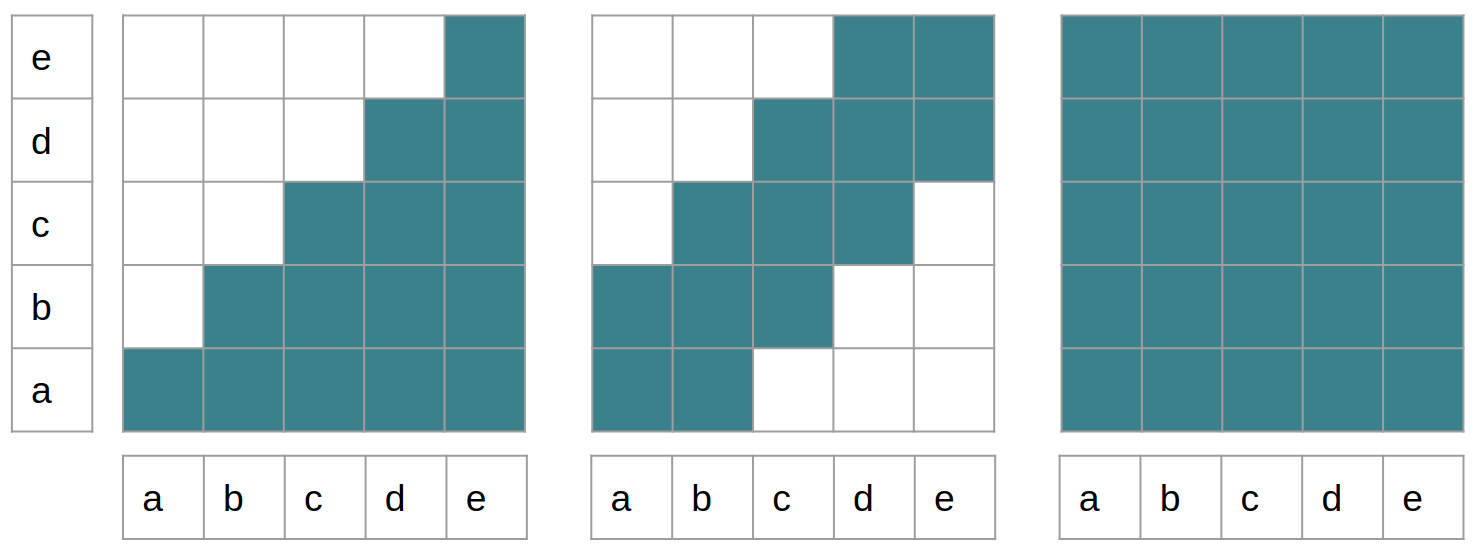
\includegraphics[width=\textwidth]{graphics/encoding.png}
\caption[Illustration of context range at each token in different encoding mechanism]{Illustration of context range at each token in different encoding mechanism. From left to right: Recurrent encoder, Convolutional encoder, Attention-based encoder. The example sequence is $[a,b,c,d,e]$ and each colored column represent the context range of the corresponding token.}
\label{fig:encoding}
\end{figure*}

The decoder works similarly to a language model as it predicts one token per time step. However, the decoder conditions its prediction on the source sequence. Therefore, the decoder takes the output of the encoder as its inputs. An Auto-regressive decoder conditions its prediction on the predictions of previous steps and the source sequence. Because all of our experiments use auto-regressive NMT, from now, a decoder is an auto-regressive decoder if there is no other specification. The decoder usually uses the same neural architecture as the encoder. However, unlike the encoder, the range of context of a token is strictly limited to its preceding tokens. Because the hidden state of the decoder is computed from the previous hidden states and the observation of the previous step, we need to initialize the $0^{th}$ hidden state $s_0$ (optional) and the $0^{th}$ token. That is why we always begin the target sequence by the token $<BOS>$, and the decoder starts predicting from the second token. For example, if $[a,b,c,d,e]$ is predicted by the decoder, the prediction of token $a$ is conditioned by source sequence $x$ and $<BOS>$; the prediction of token $b$ is conditioned by source sequence $x$ and $[<BOS>,a]$ and so on. Besides, the decoder needs a signal to stop its generative prediction. We always end a prediction by "end-of-sentence" token or $<EOS>$. Therefore, instead of predicting $[a,b,c,d,e]$, the decoder predicts $[a,b,c,d,e, <EOS>]$. Concerning the construction of hidden states, the Recurrent decoder usually initializes $s_0$ by the last hidden state of the encoder followed by a linear transformation. In contrast, the Convolutional decoder and the Attention-based decoder do not need to initialize $s_0$ as every hidden state directly accesses the predictions preceding its time step without going through its preceding state. We illustrate the difference between decoding paradigms in the figure \ref{fig:decoding}.

\begin{figure*}[htbp]
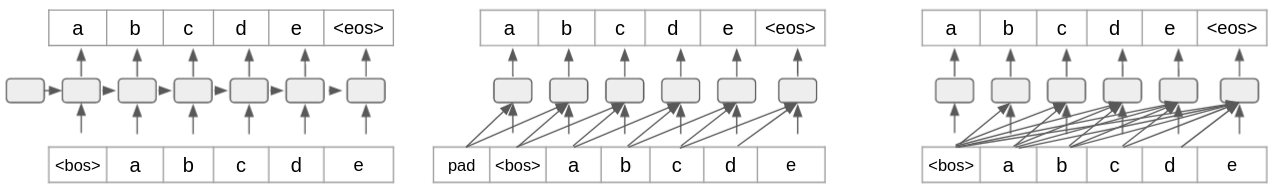
\includegraphics[width=\textwidth]{graphics/decoding.png}
\caption[Illustration of 3 most popular auto-regressive decoding paradigms]{From left to right: Recurrent decoder, Convolutional decoder, Attention-based decoder. The example sequence is $[a,b,c,d,e]$. The figure illustrates only one layer of the decoder.}
\label{fig:decoding}
\end{figure*}

NMT's Encoder/Decoder is usually a stack of multiple layers. As described above, the input source sequence is mapped to a sequence of word embeddings. This is considered as $0^{th}$ layer of the Encoder. The $i^{th}$ layer is built upon the $(i-1)^{th}$ layer by applying the same encoding mechanism, which can be recurrent layer, convolutional layer or self-attention layer, to the output of the $(i-1)^{th}$. We illustrate different multi-layer decoders in figure \ref{fig:multi-layer}. For example, \citet{Vaswani17attention} stacked 6 Transformer layers in both the encoder and the decoder of the NMT model. Deep NMT models are able to learn from very large-scale of parallel data \citep{Ott18scaling} and continually create new state-of-the-art performances. However, deep NMT models are harder to train because the gradient flow has to back-propagate through many layers. In order to prevent the gradient flow from vanishing, which happens when the value of the output of the linear transformation in some layer jumps outside the domain of the activation function, \citep{He16deep} proposes using residual connections, which replaces $f(x)$ by $f(x)+x$ where $x$ is the output of the lower layer and $f(.)$ is the transformation of the layer, to transit from the lower layers to their following layers. By using residual connections, a fraction of the gradient still reaches the lower layer and continues to propagate until the lowest layer.

Deep NMT models also suffer from Internal Covariate Shift in which the distribution of the value of each layer significantly changes due to the change of the parameters of the models. In deep network, the distribution of the value of high layers is highly affected by the parameters of the lower layers and can be dramatically shifted by a small change in the value of those parameters. Large shift can push the value of the layer to the saturation zone of activation function where the gradient is extremely small. In practice, the saturation problem can be mitigated by using the Rectified Linear Units $RELU(x) = max(x,0)$ \citep{Nair10rectified}. Recently, \citep{Ioffe15batch,Jimmy16layer} propose different normalization methods to stabilize the value of layers so that they are not easily pushed to saturation zone of activation function. In principle, Normalization methods re-scale and re-center the distribution of the value of each layer with learnable mean and learnable variance. Normalization methods prove to be very helpful in practice. For example, Layer normalization must be included in every layer of Attention-based NMT \citep{Vaswani17attention}.

\begin{figure*}[htbp]
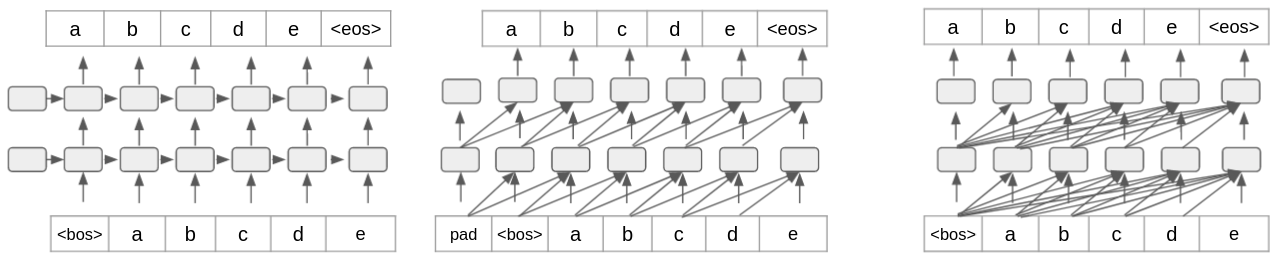
\includegraphics[width=\textwidth]{graphics/multi_layer_decoder.png}
\caption[Illustration of 3 most popular multi-layer auto-regressive decoding paradigms]{From left to right: Recurrent decoder, Convolutional decoder, Attention-based decoder. The example sequence is $[a,b,c,d,e]$. The figure illustrates only two layers of the decoder.}
\label{fig:multi-layer}
\end{figure*}

\section{Recurrent neural machine translation} \label{sec:rrn}
\nomenclature[rnn]{RNN}{Recurrent neural network}
This section reviews the very first NMT architecture, the Recurrent neural machine translation (RNMT\nomenclature[rnmt]{RNMT}{Recurrent neural machine translation}). RNMT is composed of a Recurrent encoder, a Recurrent decoder, and tables of word embeddings. Recurrent encoder and Recurrent decoder usually use the same type of Recurrent neural network (RNN) layer, such as Gated recurrent unit (GRU) and Long-short term memory (LSTM), which we will explain in the following section. RNMT is strictly auto-regressive as each hidden state in the encoder/decoder has to go through every intermediate state to assess the information of any time step before it. The hidden states of RNMT inherit the information of the order, which is an advantage before Convolutional neural machine translation (CNMT\nomenclature[cnmt]{CNMT}{Convolutional neural machine translation}) and Attention-based neural machine translation (ANMT\nomenclature[anmt]{ANMT}{Attention-based neural machine translation}), from this encoding paradigm. However, a lack of straightforward access to positions of the input sequence causes many difficulties in the training of RNMT.

\subsection{GRU, LSTM layers}
\nomenclature[gru]{GRU}{Gated recurrent unit}
\nomenclature[lstm]{LSTM}{Long-short term memory}
Gated recurrent unit (GRU) and Long-short term memory (LSTM) are the two most popular layers in the group of Recurrent neural network. They follow the auto-regressive paradigm by constructing the hidden states one by one as follows
\begin{equation}
\begin{array}{rcl}
h^l_t = f(h^{l-1}_t, h^l_{t-1})
\end{array}
\end{equation}
where $h^{l-1}_t$ is the hidden state at time step $t$ of the $(l-1)^{th}$, the $0^{th}$ layer is the sequence of word embeddings; the mapping f can be GRU cell or LSTM cell, which will be explained below.

LSTM was first introduced by \citet{Hochreiter97long}. It uses 4 gating functions including input gate i, output gate o, forget gate f and memory cell c. At each time step t, the contextualized embedding $h_t$ is computed as follows
\begin{equation}
\label{eq:lstm}
\begin{array}{rcl}
f_t &=& \sigma_g (W_f h^{l-1}_t + U_f h_{t-1} + b_f),\\
i_t &=& \sigma_g (W_i h^{l-1}_t + U_i h_{t-1} + b_i),\\
o_t &=& \sigma_g (W_o h^{l-1}_t + U_o h_{t-1} + b_o),\\
\tilde{c}_t &=& \sigma_c (W_o h^{l-1}_t + U_o h_{t-1} + b_o),\\
c_t &=& f_t \odot c_{t-1} + i_t \odot \tilde{c}_t,\\
h_t &=& o_t \odot \sigma_h(c_t),\\
\end{array}
\end{equation}
where $\sigma_g$ is the sigmoid function, $\sigma_c$ is the hyperbolic tangent function, $\sigma_h$ is either the hyperbolic tangent function or the identity function and $\odot$ is the element-wise multiplication. These functions are applied element-wise to intermediate vectors in the equations.

The motivation behind this highly complex structure is to stabilize the exploding/diminishing gradient flow \citep{Pascanu13onthe} conducted by back-propagation through time (BPTT \nomenclature[bptt]{BPTT}{Back-propagation through time}) \citep{Hochreiter97long}. The second architecture GRU, which was proposed by \citet{Cho14properties}, mitigates the complexity of LSTM by using only three gates as follows.
\begin{equation}
\label{eq:gru}
\begin{array}{rcl}
z_t &=& \sigma_g (W_z h^{l-1}_t + U_z h_{t-1} + b_z)\\
r_t &=& \sigma_g (W_r h^{l-1}_t + U_r h_{t-1} + b_r)\\
\hat{h}_t &=& \sigma_h (W_h h^{l-1}_t + U_h (r_t \odot h_{t-1}) + b_h)\\
h_t &=& (1-z_t)\odot h_{t-1} + z_t \odot \hat{h}_t\\
\end{array}
\end{equation}
Where $\sigma_h$ is a hyperbolic tangent function while other notations are the same as in the equations \ref{eq:lstm}.
\subsection{RNN encoder}
RNN encoder uses LSTM or GRU layer to encode the source sequence. RNN encoder can use more than one layer to capture more fine-grained language representation \citep{Li20shallow}. The $0^{th}$ layer is a sequence of word embeddings, which are extracted from the look-up table of the source side using the indices provided by the source sequence. 

\subsubsection{Bidirectional RNN encoder}
Unlike the decoder, the encoder is not obliged to process the input sequence from left to right. Effectively, the context of one token in the source sequence contains not only its preceding neighbors but also its following neighbors. Therefore, encoding the source sequence from left to right is not enough to cover the context of each token. To increase the coverage of contextualized embedding, the encoder process the source sequence both from left to right and from right to left at the same time therefore the encoder becomes a bidirectional encoder. Bidirectional encoding results in two sequences of contextualized embeddings; the encoder simply combines two contextualized embeddings of a token into one real vector via either concatenation or summation. The resulting contextualized embedding captures information of every word in the source sequence around its corresponding token. 
\subsection{RNN decoder}
RNN decoder predicts the target sequence from left to right, one token per time step. It initializes the $0^{th}$ hidden state by zero vector or a linear transformation of the last hidden state of the last layer of the encoder. The following section will discuss on an import component of the NMT model, which attention mechanism. As the hidden representation of the decoder at each step is computed as follow
\begin{equation}
s_i = g(s_{i-1},y_{i-1},c_i),
\end{equation}
where $c_i$ is context vector. $c_i$ is computed via attentional mechanism using $s_i$ and $Enc(x)$, which will be explained in Section \ref{ssec:attention}.

The prediction probability will be computed as follow
\begin{equation}
p(y_i|s_i,y_{i-1},c_i) = softmax(Dense(t_i))_{y_i}
\end{equation}
where $y_i$ is an index of the target vocabulary, $Dense$ is a dense layer, whose output is of dimension $|\Sigma_y|$, and $t_i$ is compute as follow
\begin{equation}
\begin{array}{rcl}
t_i &=& \big[ max\big\{ \tilde{t_{i,2j-1}}, \tilde{t_{i,2j}} \big\} \big]^{T}_{j=1,\cdots,d}, \\
\tilde{t}_i &=& U_0 s_{i-1} + V_0Emb(y_{i_1}) + C_0c_i,
\end{array}
\end{equation}
where $Emb(y_{i-1})$ is the word embedding of the token $y_{i-1}$, $U_0 \in \mathbb{R}^{2l\times d}$, $V_0 \in \mathbb{R}^{2l\times d'}$, and $C_0 \in \mathbb{R}^{2l\times d}$ in case uni-directional encoder and $C_0 \in \mathbb{R}^{2l\times 2d}$ in case bi-directional encoder.
\subsubsection{Attentional mechanism \label{ssec:attention}}
An attentional mechanism consists of 3 components: Query vectors, Key vectors, and Value vectors. Given a sequence $Q_i$, $i \in [1 \cdots n]$, $K_j$, $j \in [1 \cdots m]$ and $V_j$, $j \in [1 \cdots m]$, the results
of the attentional mechanism composed by those vectors will be as follow
\begin{equation}
Attention(Q,V,K)_i = \displaystyle{\mathop{\sum}_{j=1}^{m}} \frac{exp(sim(Q_i,K_j))}{\displaystyle{\mathop{\sum}_{p=1}^{m}}exp(sim(Q_i,K_p))}*V_j, i \in [1, \cdots, m],
\end{equation}
where the function $sim(x,y)$ can be the standard dot product $<x,y>$ \citep{Vaswani17attention}, a generalized dot product $<x,W_a*y>$ or $<v_a, tanh(W_a*[x,y])>$ \citep{Luong15stanford, Bahdanau15learning}.

The attentional mechanism manages and quantifies the dependence between the input sequence and the output sequence (e.g., source contextualized embeddings and target contextualized embeddings), or the input sequence itself (e.g., self-attention layers in Transformer \citep{Vaswani17attention}). In the RNN MT model, the attentional mechanism is used to capture the dependence of each token in the target sequence on the tokens in the source sequence. For example, \citet{Bahdanau15learning} computed a context vector at $i^{th}$ time step in the decoder as follows
\begin{equation}
\begin{array}{rcl}
c_i &=& \sum_{j} \alpha_{ij} h_j, \\
\alpha_{ij} &=& \frac{exp(e_{ij})}{\sum_{k}exp(e_{ik})}, \\
e_{ik} &=& sim(s_{i-1},h_k),\\
\end{array}
\end{equation}
where $h_j$ is the output of the last layer of the encoder, $s_{i-1}$ is the hidden state at the $(i-1)^{th}$ time step of the last layer of the decoder. 

%This context vector will be used to compute the hidden state at $i^{th}$ position by the attentional mechanism improves the translation quality of very long sequences. Indeed, the context vector produced by the RNN encoder struggles to capture all the dependence between tokens of the input sequence because it lacks the direct links between 2 tokens. The information of a token vanishes while the encoder moves toward the far ending of the input sequence. The same problem happens with the decoder when it decodes the context vector into the output sequence. The attentional mechanism provides the direct links from each output token to any input token, allows the decoder to capture the information of any input token regardless of its position.

\section{Convolutional neural machine translation} \label{sec:cnn}
\nomenclature[cnn]{CNN}{Convolutional neural network}
The convolutional neural network was successfully applied to the MT task in the work of \citet{Ghering17convolutional} that outperformed the current state-of-the-art performance of the RNMT. As we mentioned in the previous section, Convolutional neural machine translation (CNMT) does not construct the hidden states iteratively in one direction. The model considers the sequence as an image, of which each column of pixels is a word embedding, and applies convolutional kernels on it. Therefore, the CNMT is much faster than the RNMT. We give the detail of the Convolutional encoder and Convolutional decoder in the following sections.
\subsection{Convolutional encoder}
Concretely, each layer of Convolutional encoder contains a one dimensional convolution kernel followed by a non-linear activation function. We denote $h^l_i$ the $i^{th}$ hidden state of the $l^{th}$ layer. Those hidden states are computed as follows
\begin{equation}
\begin{array}{lcr}
h^l_i = v\bigg( W^l \big[h^{l-1}_{i-\frac{k}{2}}, \cdots, h^{l-1}_{i+\frac{k}{2}} \big] + b_w \bigg) + h^{l-1}_{i},
\end{array}
\end{equation}
where $W^l \in \mathbb{R}^{2d \times kd}$, $b_w \in \mathbb{R}^{2d}$, d is the dimension of hidden states as well of word embeddings, k is the width of the kernel, the activation function v is Gated Linear Unit \citep{Ghering17convolutional} as follows
\begin{equation}
\begin{array}{lcr}
v([A,B]) = A \odot \sigma(B),
\end{array}
\end{equation}
where $\odot$ is element-wise multiplication, $\sigma$ is sigmoid function.
\subsection{Convolutional decoder}
Unlikely the Convolutional encoder, in which each hidden states has access to its left and right neighbors, the decoder only allows left accesses to avoid conditioning the predictions on the following tokens, which remain unknown before the prediction during the inference. Therefore, \citet{Ghering17convolutional} appended $k-1$ padding tokens in the left side of the output sequence, e.g $PAD$, $PAD$,$ <BOS>$,$je$,$t'$,$aime$ for convolution kernel of size 3 so that $\big[ PAD, PAD, <BOS>\big]$ predicts $je$, $\big[ PAD,<BOS>,je\big]$ predicts $t'$ and so forth.
The Convolutional decoder also uses an attention mechanism to improve the performance of long sentences. \citet{Ghering17convolutional} proposed a version slightly different from ones of \citet{Luong15stanford, Bahdanau15learning}. For each $l^{th}$ decoder layer, the query will be a combination of the hidden state $h^l_i$ and the word embedding of the previous token $g_i$ as follows
\begin{equation}
\begin{array}{rcl}
Q^l_i = W^l_d h^l_i + b^l_d + g_i.
\end{array}
\end{equation}
The keys are still the hidden states of the last layer of the encoder $z^u_j$. The values are the combinations of the hidden states $z^u_j$ and the word embedding $e_j$ as follows
\begin{equation}
\begin{array}{rcl}
V^l_j = z^u_j + e_j.
\end{array}
\end{equation}
The score attention is the dot product between the query vector and the key vector followed by the softmax function as follows
\begin{equation}
\begin{array}{rcl}
\alpha_{ij}=\frac{exp(Q^l_i \cdot z^u_j)}{\sum_{t=1}^m exp(Q^l_i \cdot z^u_t)}.
\end{array}
\end{equation}
The context vector $c^l_i$ will be as follow
\begin{equation}
c^l_i = \sum_{j=1}\alpha_{ij}V^l_j
\end{equation}
Once $c^l_i$ has been computed, it is simply added to the output of the corresponding decoder layer $h^l_i$.
\subsection{Positional embedding}
\citet{Ghering17convolutional} proposed using embeddings corresponding to each position of the input sequence. The purpose is to equip the CNMT model with a sense of order as the Convolution kernel does not take into account the order of tokens in the input sequence. Effectively, if we interchange the position of tokens outside the window of the kernel, the value of the hidden state does not change. Positional embeddings are real value vectors having the same dimension as word embeddings. Positional embeddings are added to word embeddings of the corresponding position before passing to the first layer.

\section{Attention-based neural machine translation} \label{sec:transformer}
Transformer architecture was first introduced by \citet{Vaswani17attention} and has quickly become the state-of-the-art architecture not only in MT but also in language modeling (LM)  \citep{Devlin19bert,Brown20language,Conneau19cross}, text summarization \citep{Zhang20pegasus} etc. The Transformer model's power relies on the attentional mechanism, which was discussed in the previous section \ref{ssec:attention}. The Transformer model consists of a fully attention-based encoder and decoder. 
\subsection{Transformer encoder}
\label{ssec:transformer-enc}
The Transformer encoder consists of layers made of a multi-head self-attention sub-layer followed by a position-wise fully connected feed-forward network. The multi-head self-attention sub-layer is an extension of the self-attention sub-layer and is described by the following equation
\begin{equation}
\begin{array}{rcl}
MultiheadAttention\big( Q,V,K \big) &=& Concat \big[ head_0, \cdots , head_h \big] W_0\\
head_i &=& Attention \big( QW_i^Q, VW_i^V, KW_i^K \big),\\
\end{array}
\end{equation}
where $W_i^Q, W_i^V, W_i^K \in \mathbb{R}^{d_k \times d_h}$ with $d_h \times h = d_k$, $d_k$ is the dimension of word embedding space and also the size of Transformer model. Unlike the version \eqref{eq:self-att} in Section \ref{ssec:attention}, the attentional mechanism is simply as follows,
\begin{equation}
Attention\big( Q, V, K \big) = Softmax\big(\frac{Q K^T}{\sqrt{d_k}} \big) V.
\end{equation}
The feed-forward network is designed as follows
\begin{equation}
FFN(x) = ReLu(xW_1+b_1)W_2+b_2,
\end{equation}
where $W_1 \in \mathbb{R}^{d_k \times d_b}$,$W_2 \in \mathbb{R}^{d_b \times d_k}$,$b_1 \in \mathbb{R}^{d_b}$,$b_2 \in \mathbb{R}^{d_k}$.
The final detail is that the output of each sub-layer has to pass through a Layer-Normalization sub-layer \citep{Jimmy16layer}. In conclusion, the contextualized embedding of the $l^{th}$ layer of the Transformer encoder will be as follows
\begin{equation}
\begin{array}{rcl}
\tilde{h}^l &=& LN\bigg(Multihead\big(h^{l-1}, h^{l-1}, h^{l-1}\big) + h^{l-1}\bigg), \\ 
h^l &=& LN\bigg(FFN\big(\tilde{h}\big) + \tilde{h}\bigg),
\end{array}
\label{eq:self-att}
\end{equation}
where $LN$ is a Layer-Normalization sub-layer.
\subsection{Transformer decoder}
The Transformer decoder consists of layers made of a multi-head self-attention sub-layer followed by a multi-head cross-attention sub-layer then by a position-wise fully connected feed-forward network. The multi-head self-attention sub-layer and the feed-forward network have the same design as those in the Transformer encoder. The multi-head cross-attention sub-layer of the $l^{th}$ layer of the decoder uses the output of the last layer of the encoder as keys and values, the output of the $l^th$ self-attention sub-layer as queries
\begin{equation}
\begin{array}{rcl}
\tilde{s}^l &=& LN\bigg( Multihead\big( s^{l-1},s^{l-1},s^{l-1} \big) + s^{l-1} \bigg), \\
\bar{s}^l &=& LN\bigg( Multihead\big( \tilde{s}^l, h^u, h^u \big) + \tilde{s}^l \bigg), \\
s^l &=& LN\bigg( FFN\big( \bar{s}^l \big) + \bar{s}^l \bigg), \\
\end{array}
\end{equation}
where $s^l$,$s^{l-1}$ are the outputs of the $l^{th}$ and $(l-1)^{th}$ layers of the decoder respectively, $h^u$ is the output of the last layer of the encoder.

In order to prevent the future information in the decoder, at each time step $i^{th}$, the attention scores of tokens at positions after $i^{th}$ are masked by zero.

\subsection{Positional embedding}
Similar to the Convolutional encoder/decoder, the Transformer encoder/decoder does not respect the order of tokens as it fully connects every pair of tokens in parallel. In order to represent the position of tokens in the sequence, \citet{Vaswani17attention} proposed the use of positional embedding. Unlike \citet{Ghering17convolutional}'s positional embedding, this version is not parameterized as given the size of word embedding $d_k$ , the positional embedding of position $i^{th}$ is defined as 
\begin{equation}
\begin{array}{rcl}
PE\big(pos,2i\big) &=& sin \big( \frac{pos}{1000^{\frac{2i}{d_k}}} \big)\\
PE\big(pos,2i+1\big) &=& cos \big( \frac{pos}{1000^{\frac{2i}{d_k}}} \big).\\
\end{array}
\end{equation}
The positional embedding will be added to the corresponding word embedding of the $i^{th}$ token of the input sequence.
\section{Training NMT models} \label{sec:train}
The purpose of training NMT model is to find optimal values for its parameters so that the error of the model are minimal in the testing. To learn these optimal values, we need 3 type data sets including training set, validation set, and testing set. Training set is used to optimize the model's parameters via statistical learning algorithms such as Maximum likelihood estimation (MLE\nomenclature[mle]{MLE}{Maximum likelihood estimation})\citep{Baum87Supervised}. Testing set is used to evaluate the model once it's optimized. The performance on the testing set shows us how good the model is and is used to compare different models. Validation set is not used to learn the model's parameters nor to evaluate the model but to prevent the "over-fitting" of the optimization. Effectively, an NMT model can be trained until very small error in the training set but has poorer performance in the testing set than another NMT model which is trained with early stopping criteria. During the training, the model is evaluated on the validation set for every $K$ iterations. The learning is represented by 2 learning curves, including the error on training set and the error on the validation set. The stopping criteria is whether the validation error does not improve after a predetermined number of consecutive evaluations.

Concerning the optimization of the model on the training set, we usually use MLE, i.e.
\begin{equation}
\hat{\theta} = \displaystyle{\mathop{argmax}\mathop{\sum}_{x,y \in \mathit{D}}}log P(y|x;\theta),
\label{eq:mle}
\end{equation}
where $\mathit{D}$ is the sampling distribution of the training data.
MLE is equivalent to minimizing the cross-entropy loss
\begin{equation}
\begin{array}{rcl}
L_{CE}(\theta,\mathit{D}) &=& -\displaystyle{\mathop{\sum}_{(x,y) \in \mathit{D}} \mathop{\sum}_{i}^{l_y}}log P(y_i|y_{<i},x;\theta), \\
\hat{\theta} &=& \displaystyle{\mathop{argmax}} L_{CE}(\theta).
\end{array}
\end{equation}
In order to optimize this function, we often use the gradient descent method, which is one of the oldest approaches in the Optimization area \citep{Cauchy1847method}. The gradient is computed by back-propagation algorithm \citep{Rumelhart88learning}. Like many deep learning models, the NMT model is usually trained with a massive amount of data that makes the gradient descent method is not computationally plausible. Therefore, stochastic gradient descent (SGD\nomenclature[sgd]{SGD}{Stochastic gradient descent}) is proposed to mitigate the computational burden of large-scale models \citep{Herbert51stochastic,Kiefer52stochastic,Bottou10large}. Instead of calculating the gradient of the loss over every training examples, SGD samples a batch of examples from training set, calculates the gradient of the loss over this batch, then updates the parameters according to this gradient.
\subsection{Tips and tricks in training an NMT model}
Deep Neural networks are usually very hard to train. Effectively, back-propagation through time in RNMT usually creates exploding or vanishing gradients \citep{Pascanu13onthe,Glorot10understanding}. Gradient clipping \citep{Pascanu13onthe}, Truncate back-propagation \citep{Jaeger02tutorial} are proposed to mitigate this problem.

Large NMT models are easily over-fitted to training data. \citet{Srivastava14Dropout} proposed randomly freezing a subset of parameters during one training iteration, which prevents the whole model from being fitted to one example. We could interpret Dropout as an ensemble method that allows training many sub-networks in one training and ensembles them in testing. In practice, Dropout is essential to train neural models in general. 

Besides, the Log-likelihood maximizing \eqref{eq:mle} assumes that a ground-truth label is far more likely than all other labels, excessively discriminates between the likelihood of training examples and the likelihood of language that does not appear during training. The Log-likelihood maximizing can result in over-fitting to the training data, reducing the model's generalization in testing.

\section{Inference with an NMT model} \label{sec:inference}
An NMT model translates a source sentence $x$ by searching the target sequence y that gives the highest probability conditioned on $x$,
\begin{equation}
\hat{y} = \displaystyle{\mathop{\argmax}}. P(y|x;\theta)
\end{equation}
However, the search space of $y$ is of infinite dimension, causing the implausibility of the exact search. Beam search \citep{Och98improving} is the most common inference algorithm in Neural Machine Translation and Statistical Machine Translation. For autoregressive NMT models, a single output token is produced at each inference step $j$. The prediction at step $j$ is conditioned by $x$ and the partial translation hypothesis up to step $j$
\begin{equation}
\hat{y}_j = \displaystyle{\mathop{\argmax}_{y_j \in \Sigma_y}} P(y_j|y_{<i},x,\theta).
\end{equation}
Beam search tracks K most probable translation hypothesis. Beam search starts with K empty hypotheses, which are initialized by "begin of sentence" token $<BOS>$. In the $j^{th}$ inference step,
for the $n^{th}$ partial hypothesis $[y^{n}_{<j}]$, the top-K most probable tokens according to $P(.| y_{<j},x;\theta)$ are picked and appended to the current hypothesis
\begin{equation}
\hat{y}^n_j \in \displaystyle{\mathop{Top_{K}}_{y_j \in \Sigma_y}} P(y_j|y_{<j},x,\theta).
\end{equation}
The search space, therefore, is extended to $K*K$ hypotheses. Beam search selects only the top $K$ hypotheses from these $K*K$ hypotheses. It stops extending an hypothesis when $<EOS>$ is predicted or  the hypothesis reaches the predefined length limit. 

Beside the left-to-right decoding, there are several variant decoding direction including non-monotonic decoding \citep{Welleck19non}, non auto-regressive decoding \citep{Jiatao17non}, and synchronous bidirectional decoding \citep{Zhou19synchronous}. Because the decoding algorithms are not included in this research topic, we would like to be limited to this brief description.
\nomenclature[eos]{EOS}{end-of-sentence}
\section{MT evaluation}
The evaluation of MT systems can be done automatically by comparing n-grams of generated translations and n-grams of gold references. The most popular MT metric is BLEU \citep{Papineni02bleu}. Recently, \citet{Post18A} proposed standardizing hypotheses of MT systems before calculating BLEU metric. 

BLEU is computed on corpus-level, i.e., it compares a corpus of hypotheses and the corpus of references. BLEU score is the geometry average of n-gram precisions, including 1-gram, 2-grams, 3-grams and 4-grams weighted by brevity penalty (BP)
\begin{equation}
BLEU = BP exp(\frac{1}{4}\sum_{i=1}^4log p_i).
\end{equation}

The n-gram precision $p_n$ is computed as follows
\begin{equation}
p_n = \frac{\sum_{hyp \in hyps}\sum_{n\text{-}gram \in n\text{-}grams} min(Count(Ref,n\text{-}gram), Count(hyp, n\text{-}gram))}{\sum_{hyp \in hyps}\sum_{n\text{-}gram \in n\text{-}grams} Count(Ref,n\text{-}gram)},
\end{equation}
Where $Count(C,g)$ is the number of occurrences of the n-gram $g$ in the corpus $C$.

The Brevity penalty computed as follows
\begin{equation}
  BP =
    \begin{cases}
      1 & \text{if $|c| > |r|$ }\\
      exp(1-\frac{|r|}{|c|}) & \text{otherwise}.
    \end{cases}       
\end{equation}
Where $c$ is the total length of the hypothesis corpus, $r$ is the total length of the reference corpus. The Brevity penalty assures that a high-scoring candidate translation must also match the reference translations in length.








































	\chapter{Machine translation (multi-)domain adaptation's review} \label{chap:revisting}
Machine translation (multi-)domain adaptation has a long history as the area has been actively studied for almost two decades and is still being explored to communicate many languages in many fields better. The earliest domain adaptation methods were explored for SMT systems. Recently, most of the effort has been made to adapt better NMT systems to domains for NMT has surpassed SMT to be state-of-the-art architecture. In this chapter, we would like to do our best to give a thorough literature review of the problem. More precisely, we formally point out 4 principle cases of (multi-)domain adaptation and revise the approaches for each case. We also adopt the survey of \cite{Chu18asurvey} in our review.

We divide this chapter into five sections. In the first section \ref{sec:domain}, we would like to discuss how we usually define a domain, how translations differ between domains and the importance of domain adaptation in real applications. In the second section \ref{sec:multi-facet} we would like to regroup two notions, domain adaptation, and multi-domain adaptation, then divide the large problem MT (multi-)domain adaptation into four sub-problems. We dedicate four following sections to those sub-problems. In each of the four following sections, we review groups of approaches, according to \citet{Chu18survey}, that match the requirement of the corresponding problem.
\section{What is a domain?}
\label{sec:domain}
In a classical machine learning context such as binary classification problem, \citet{Shai10A} defined a domain by a pair consisting of a distribution $\mathcal{D}_x$ on inputs $\mathcal{X}$ and a labeling function $f: \mathcal{X} \rightarrow [0,1]$. In machine translation context, the labeling function will be $f: \mathcal{X} \rightarrow \mathcal{Y}$ where $\mathcal{X}$ and $\mathcal{Y}$ are the set of sentences of the source language and the target language respectively. Denote 2 different domains, $\big( \mathcal{D}_S, \mathcal{F}_S \big)$ and $\big( \mathcal{D}_T, \mathcal{F}_T \big)$. Domain adaptation is required when we train a machine learning model (statistical or neural) with data generated by $\big(\mathcal{D}_S, \mathcal{F}_S \big)$ but test it with data generated by $\big(\mathcal{D}_S, \mathcal{F}_S \big)$. In principle, there is no guaranty that the model performs well in the second domain. However, we could aim to exploit some sharing knowledge between the two domains; for example, \citet{Blitzer06Domain} explored pivot features, which are features that frequently occur in the two domains and similarly contribute to the predictions in both domains. The context of machine translation is much more complicated than binary classification as the label is a structured sequence of symbols that has to satisfy both the adequacy according to the source sequence and the fluency according to the target language. \cite{Wees15Whats,Wees17Whats} identified the following elements of text, which influence the translation the most.
\begin{itemize}
	\item Topic: the subject of the text such as medical, news, IT, or religious. A topic owns its own specific vocabulary, terminologies. These items can not be transferred between distant topics such as medical and religion.
	\item Genre: the purpose of the text such as education, talk, report, or instruction. It identifies groups of texts that share a common form of transmission, purpose, and discourse properties. We characterize genre by textual style, the structure of the text, etc.
\end{itemize}

Despite many specifications, domains share the same grammar of the corresponding language. However, the concepts such as the grammar, the textual style, or the text structure are abstract to machine translation models. MT models learn to translate from examples without being explicitly explained how to do it. They are supposed to learn this knowledge to translate, but we cannot tell whether they do it until now.

Solving the MT (multi-)domain adaptation problem is essential for deploying MT in a real context. Machine Translation has applications in many sectors, such as translating legal documents, news, scientific documents, books, movie subtitles, etc. Every domain has its own specific vocabulary, registers(formal or informal), and genres (e.g., talk, instruction). Therefore, tailoring MT models to a target domain is essential to achieve good translation in that domain. In practice, MT models (SMT, NMT) trained with domain-related data always perform much better in the domain of interest than ones trained with the same amount of less relevant data \citep{Rico13domain, Saunders21Domain}. The more domain-relevant data is available, the better the MT system performs in the target domain. However, not every domain has enough data to train an MT model. The state-of-the-art architecture ANMT will need millions of parallel sentence pairs to learn its parameters. Therefore, we have to work around the situation where there is very little data or even no data. Domain Adaptation aims to improve the performance of an MT model in low-resourced domains. Besides, multi-domain adaptation seeks to achieve the best performance in more than one domain. However, the domains of interest in multi-domain adaptation are not limited to be low-resourced domains. The motivation of having one model adapted to many domains is to optimize the storage, the training time, and the deploying time. Having one model per domain increases the storage, the time retrieving a model, and thus the translation latency. Online translation services, such as Google Translate, Systran Translate, or DL Translate, have to translate text from any possible domain while minimizing the latency of translation in order to be beneficial. In conclusion, the variety of text between fields requires domain adaptation, while fast and robust translation requires multi-domain adaptation.

\section{Machine translation (multi-)domain adaptation a multi-faceted problem}
\label{sec:multi-facet}
\subsection{From domain adaptation MT to multi-domain adaptation MT}
Even though domain adaptation and multi-domain adaptation do not have same motivation as one focuses on low-resourced domain whereas the other focuses on adapting to as many as possible domains, they can be cast under one general framework. Formally, training instances are distributed according to a mixture $\mathcal{D_S}$ such that $\mathcal{D_S}(x) = \sum_{d=1}^{n_d} \lambda^{s}(d) \mathcal{D}_d(x)$, with $\{\lambda^{s}(d), d=1 \dots n_d\}$ the mixture weights satisfying $\sum_d \lambda^{s}(d)=1$. The target domains are represented in the test distribution which is also a mixture of $\mathcal{D_T}(x) = \sum_{d=1}^{n_d} \lambda^{t}(d) \mathcal{D}_d(x)$, with $\{\lambda^{t}(d), d=1 \dots n_d\}$ the mixture weights satisfying $\sum_d \lambda^{t}(d)=1$. We assume $\mathcal{D}_d(x), d=1 \dots n_d\}$ is the support of the both source and target distribution. Domain adaptation solves the case where $\lambda^s * \lambda^t = 0$ and $\lambda^t$ is one-hot vector while multi-domain adaptation happens to solve the case where $\lambda^t$ is not one-hot vector. We illustrate this formulation in figure %\ref{fig:mdmt-lambdas}.
\begin{figure}[h]
  \centering
  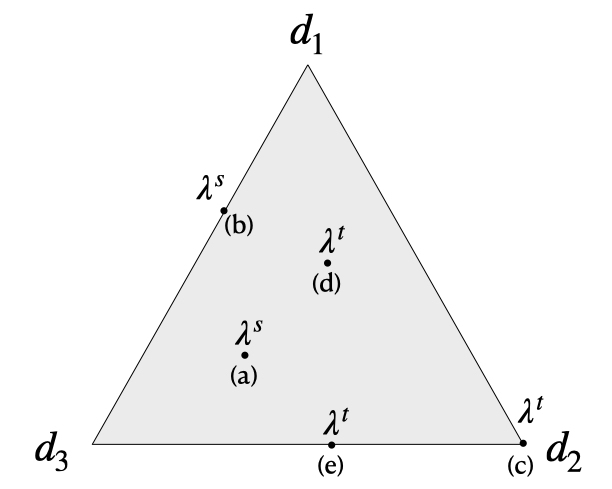
\includegraphics[width=0.5\textwidth]{graphics/mdmt-lambdas}
  \caption[Training and testing with distribution mismatch]{Training and testing with distribution mismatch. We consider just three domains, and represent vectors of mixture weights $\vlambda^{s}$ and $\vlambda^{t}$ in the 3-dimensional simplex. Training with weights in (a) and testing with weights in (c) is supervised multi-source domain adaptation to domain~2 ($d_2$), while (b)-(c) is the unsupervised version, with no training data from $d_2$; training with weights in (a) and testing with weights in (d) is multi-domain learning, also illustrated with configurations (a)-(e) (training domain $d_1$ is not seen in test), and (b)-(d)  (test domain $d_2$ is unseen in training).}
  \label{fig:mdmt-lambdas}
\end{figure}

This framework modelizes the real context closely because, in a typical setting in machine translation, we collect the most extensive collection of parallel data for the chosen language pair to achieve optimal performance for the task of interest. In such situations, the training data distribution is opportunistic. The test data distribution is determined and fixed; a key component in training is to mitigate the detrimental effects of a possible mismatch between these distributions. Training data may be a mixture of many domains such as the JRC-Acquis Communautaire corpus (\domain{law}-domain) \citep{Steinberger06acquis} or documentation for KDE, Ubuntu, GNOME and PHP from the Opus collection \citep{Tiedemann09news} (\domain{it}-domain). We also leverage a collection of data with no specific topic and genre, such as Paracrawl \citep{Banon20Paracrawl}. The testing data represent the domains of interest. In multi-domain adaptation, because there are multiple target domains, the testing is composed of multiple tests. The performance of an MT system is usually the average of its performance on these tests. However, we can access the quality of the multi-domain MT system with different priorities over target domains using weighted mean. The evaluation of multi-domain MT system should be clarified before training as early stopping criteria relies on the evaluation over validation tests.
\subsection{4 main sub-problems}
From our study on many previous works, we realize that the (multi-)domain adaptation problem is a multifaceted problem. Effectively, all the cases of (Multi-)domain adaptation can be classified into four groups by answering two following questions:
\begin{itemize}
	\item Is/Are the domain(s) of the training deterministic?
	\item Is/Are the domain(s) of the testing deterministic?
\end{itemize}
More precisely, the first question asks whether the training data is composed of a number of known domains. For example, the domain of a mixture of multiple corpora of specific topics, such as JRC-Acquis Communautaire corpus (\domain{law}-domain) and KDE (\domain{it}-domain), is well defined. However, the domains in Paracrawl \citep{Banon20Paracrawl} is unknown because it was built by crawling the content of web-sites without specifying topic or purpose. The second question asks whether the domain of the testing data is determined. If there exists a collection of text (monolingual or parallel) that defines the domain of the testing, then it is domain-deterministic and vice versa. 

Our first case of (multi-)domain adaptation \ref{sec:case1} is supervised multi-domain adaptation in which domain labels are both available in training and testing. Furthermore, the target domains in testing are included in the training. This case might be the most straightforward situation. Many approaches in multi-domain MT conducted their experiments in this setting \cite{Pham21revisiting}. 

The second case \ref{sec:case2} considers the use of the parallel data crudely collected from webs such as Paracrawl \citep{Banon20Paracrawl} or Commoncrawl \footnote{\url{https://commoncrawl.org/}}. The content of these corpora varies from many topics, but unfortunately, there is not any available domain label for sentences. Fortunately, in the second case, the target domains are known, i.e., there exist data of these domains, which can be used to adapt the model. The second case focuses on the exploitation of opportunistic text. 

The third case \ref{sec:case3} assumes a well domain-labeled training data while allowing the testing sentence from any possible domain. This case focuses on the robustness of the MT system against any possible shift distribution in testing. The third setting is very closed to real applications where the provenance of the input text is unknown. 

Finally, the last setting \ref{sec:case4} focuses on both exploiting opportunistic data in training and being robust against unknown testing distribution. We dedicate the four following sections to discuss more details of each setting.

Recently the work of \citet{Chu18survey} significantly captured the landscape of MT domain adaptation by categorizing previous methods in 2 main classes: data-centric and model-centric. The data-centric category includes methods that manipulate the training distribution to resemble the distribution of the target domain better. The model-centric methods focus on changing the architecture, modifying the training objective, and improving the inference.

According to \citet{Chu18asurvey}, the data-centric focuses on two paradigms, including 1) collecting parallel data related to the domain target, 2) creating synthetic data resembling the domain target. The first paradigm searches for similar examples to the ones of the domain target to enlarge the domain target's training data. The second paradigm aims to create pseudo examples resembling the data of the domain target. Besides the two paradigms, we propose another paradigm, which is data sampling. The data sampling paradigm consists of changing the data sampling distribution during the training course to mitigate the heterogeneity of the data size between domains and the variety of the "difficulty" of the domains. Therefore data-centric consists of 3 paradigms, including 1) data collection, 2) data synthesization, and 3) data sampling.

This taxonomy is largely adopted in MT domain adaptation's research. However, we find a naivety in this classification as it misses delivering an answer for the most ultimate question: "which method solves which problem?". We propose adding another dimension, the context of the MT adaptation problem, to form a Cartesian map of the MT (multi-)domain adaptation area. The four following sections will explain how model-centric and data-centric categories solve 4 (multi-)domain adaptation cases. We believe that this coupling of methods and cases will allow us to navigate better the (multi-)domain adaptation forest that has been growing for almost two decades. We also introduce several unexplored adaptation problems that need more research effort and other applications of existing application methods. The work of \citet{Pham21revisiting} recently gave a brief review of several well-known adaptation methods via a reevaluation with different domain adaptation cases. However, the experiments are still limited in the first case \ref{sec:case1} and the third case \ref{sec:case3} by excluding crawled corpora.

\section{Supervised (multi-)domain adaptation}
\label{sec:case1}
In the supervised (multi-)domain adaptation, the domain label is available in both training and testing. Furthermore, the domain(s) in testing is(are) available in training. In this problem, we would like to achieve a unique model that performs the best in one or many target domains, given training data from those domains and probably from other domains. This setting is the most popular situation on which multi-domain machine translation research papers focus. The first case represents the least requirement as the MT needs to achieve the best performance on the domains it learned from. The difficulty of this situation is to both exploit the proximity between domains while mitigating the interference due to inter-domain heterogeneity. Effectively, similar topics, such as legal and administrative, might improve the vocabulary coverage of each other as both domains share the same specific terminologies. However, distant topics, such as religion and IT might confuse the MT system when sharing the same parameters. In the following sections, we will discover how model-centric methods and data-centric methods solve this case.
\subsection{Model-centric}
In the case of the supervised multi-domain adaptation, model-centric methods focus on adding domain-specified parameters to reduce the interference between domains while keeping the number of parameters small. The simplest methods use domain tags. For example, \citet{Kobus17domain} proposed appending a special token to each source sequence indicating its domain such as $<Domain=IT>$ and train the NMT model with this format. However, this format requires domain tags in testing; hence we have to predict them if the source sentences are from an unknown origin. \cite{Britz17effective} originally proposed appending domain tag to the target sequence so that the decoder will predict the domain in which it will generate the translation. Instead of using domain tag, \citep{Kobus17domain, Pham19generic} proposed using domain embedding to incorporate the domain information into the context of the translation. \citet{Kobus17domain} concatenated an embedding of small size (e.g., 4) to the embedding of each token in the input sequence. Each small embedding corresponds to a domain. Instead of using the same domain embedding for the tokens in the same domain \citet{Pham19generic} used lexicalized domain representation, which is a small embedding correspond to the domain and the token. Besides domain embedding, we can use domain-specified layers that can be plugged between 2 consecutive layers of the NMT model without changing the architecture. There are 2 types of plug-in layers: 1) residual adapter \citep{Bapna19simple, Pham20Study} and 2) learning hidden unit contribution \citep{Vilar18learning}. Residual adapters were first introduced by \citet{Rebuffi17learning} in computer vision. \citet{Bapna19simple} proposed this fine-tuning paradigm for domain adaptation. They introduced a new version of residual adapter composed of 2 linear projections and the ReLU activation function. The adapters are plugged into the NMT model as follow
\begin{equation}
\begin{array}{rcl}
h_{enc/dec}^l = h_{enc/dec}^{l} + ADAP_{enc/dec}^l(h_{enc/dec}^{l})
\end{array}
\end{equation}
where $ADAP_{enc/dec}^l$ is the adapter corresponding to the $l^{th}$ layer of the encoder/the decoder. \cite{Pham20Study} studied the use of the residual adapters for multi-domain adaptation and propose several techniques, including regularization, gating mechanism, to improve the robustness of the model. The learning hidden unit contribution (LHUC \nomenclature[lhuc]{LHUC}{Learning hidden unit contribution}) method was proposed by \cite{Vilar18learning} to adapt an NMT model to a domain. The author applied an LHUC layer to the model as follow
\begin{equation}
h_{enc/dec}^l = h_{enc/dec}^{l} \odot a(\rho^{l}_{enc/dec})
\end{equation}
where $\rho^{l}_{enc/dec}$ is the adapter corresponding to the $l^{th}$ layer of the encoder/the decoder and $\rho^{l}_{enc/dec} \in \mathbb{R}^d$. $a(.)$ is a scaled
element-wise sigmoid function.
$$a(x) = \frac{2}{1+e^{-x}}$$
Residual adapter and learning hidden unit contribution layer adapt a pretrained model without changing its parameters. 

While the previous methods aim to discriminate domains to reduce the interference,\cite{Britz17effective} was motivated to learn hidden representations that are invariant between domains. More precisely, the authors use a binary classifier that takes the output of the encoder as input to distinguish the source sequences of 2 source domains. They inverse the sign of the gradient corresponding to the loss of the classifier to confuse it, i.e., making the hidden representation of the encoder invariant between 2 domains. This technique is related to A-distance, which is a measure of similarity between two probability distributions. \cite{Ben07analysis} showed that the A-distance between the
source and target distributions is a crucial part of an upper generalization bound for domain adaptation. They hypothesized that it should be difficult to discriminate between the source and target domains to have a good transfer between them because
this would imply similar feature distributions. \cite{Zeng18multidomain}'s work was also inspired by this idea. However, instead of forcing the encoder's output to be invariant between domains, the authors focus on extracting domain-agnostic features and domain-specific features from the output of the encoder and feeding the features to the decoder. To do that, they use two different non-linear transformations, which map a hidden representation to two vectors of the same size. Then, they apply one domain classifier on each extracted feature vector. The domain-agnostic feature vector is trained to confuse its corresponding classifier, whereas the domain-specific feature vector is trained to facilitate its classifier.

\cite{Michel18extreme} adapted a pretrained model to a multi-user personalized model by fine-tuning the
bias of the output softmax to each particular user of the MT system. The number of additional parameters is $|S| \times |\Sigma_y|$, in which $S$ is the set of the users. The author reduces the size of the bias matrix $B \in \mathbb{R}^{|S| \times |\Sigma_y|}$, whose each row is a bias vector of one user, by factoring it into lower dimension representation, i.e.
\begin{equation}
\begin{array}{rcl}
B &=& S \times \tilde{B}, \\
&where& \\
S & \in & \mathbb{R}^{|S| \times r}, \\
\tilde{B} & \in & \mathbb{R}^{r \times |\Sigma_y|}.
\end{array}
\end{equation}

\citet{Jiang20Multi}'s work was inspired by the mixture of expert paradigm. Their novel model is based on Transformer architecture \citep{Vaswani17attention} as they integrate a domain-mixing mechanism to the multi-head attention layer. As we explained in Section ~\ref{ssec:transformer-enc}, each head of multi-head attention layer is computed as follow
\begin{equation}
head_i = Attention \big(QW_i^Q, VW_i^V, KW_i^K \big).
\end{equation}
Suppose that there are $K$ domains, at the $i^th$ head, for each query, key and value component, there are $K$ transformation matrix $W_{i,j}^Q | j \in [1,K]$, $W_{i,j}^K | j \in [1,K]$, $W_{i,j}^V | j \in [1,K]$ respectively. The domain-mixing mechanism is applied on query, key and value components as follow
\begin{equation}
\begin{array}{rcl}
Q_i^t &=& \sum_{j=1}^K Q^tW_{i,j}^Q*\mathit{D}_j(x_t),\\
K_i^t &=& \sum_{j=1}^K K^tW_{i,j}^K*\mathit{D}_j(x_t),\\
V_i^t &=& \sum_{j=1}^K V^tW_{i,j}^V*\mathit{D}_j(x_t),\\
head_i &=& Attention \big( Q_i, K_i, V_i\big),
\end{array}
\end{equation}
where the subscript $t$ indicates the position of the vector in the sequence of hidden representations, $\mathit{D}(x_t) \in \mathbb{R}^{K}$ is the domain proportion of the corresponding token $x_t$. The proportion of domains of a token is computed by a domain classifier, that take the input embedding of that token as input. The novel model adapt the hidden representation of a token to a domain to which the token likely belongs. Therefore, the model is able to discriminate domains in domain-specific tokens while transfering knowledge between domains in domain-agnostic tokens. However, the size of the model is proportional to the number of domains, which is not practical in the real applications. However, in our opinion, the idea can be applied to lightweight adapter or learning hidden unit contribution layer.

Besides the model-centric methods related to the architecture, multi-task training is another solution to the supervised (multi-)domain adaptation problem. 

We illustrate several well-known model-centric methods for the supervised domain adaptation problem in Figure~\ref{fig:model-centric-case1-case2}.
\begin{figure}[htbp]
\begin{subfigure}{1.0\textwidth}
  \centering
  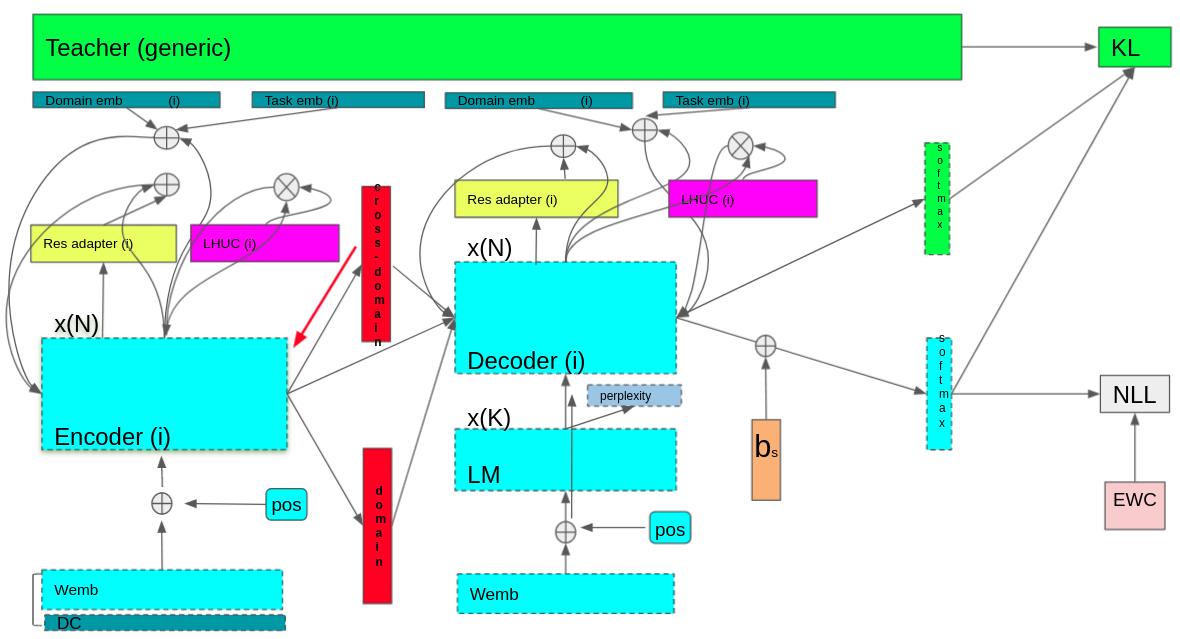
\includegraphics[width=1.0\textwidth]{graphics/supervised_mdmt}
\end{subfigure}
\newline
\begin{subfigure}{1.0\textwidth}
  \centering
  \fbox{\begin{tabular}{ll}
\textcolor{red}{$\blacksquare$} & \citep{Zeng18multidomain} \\
\textcolor{violet}{$\blacksquare$} & \citep{Vilar18learning} \\
\end{tabular}}
\end{subfigure}
\caption[Model-centric's brief overview]{Each color different from the bleu corresponds to one model-centric method. The bleu represents the NMT model.}
\label{fig:model-centric-case1-case2}
\end{figure}

\subsection{Data-centric}
\subsubsection{Data sampling}
In supervised multi-domain adaptation, data sampling approaches aim to balance the contribution of each domain to the final model. In an opportunistic multi-domain training data, the data size of each domain vary from few thousands examples to millions examples. In a trivial mixture of data, small domains are usually excessively under-sampled causing a sub-optimal performance in average. However, if we equally sample data from every domain, the NMT model is easily over-fitted in the small domains. Therefore, finding optimal sampling distribution of domains is essential. \cite{Wang20balancing} proposed parameterizing the probability of sampling data from a domain and learned this probability via REINFORCE algorithm \citet{Williams92simple} using rewards computed from cosine-similarity between the gradient over in-domain training data and the gradient over dev-sets' data. We compare this technique to our approach in chapter \fyTodo{add reference of chapter MDAC here}.

Other data-centric methods, that does not take into account the domains of the training data will be discussed in Section ~\ref{ssec:case-2-data}.
\section{Non domain-deterministic training, domain-deterministic testing}
\label{sec:case2}
In this situation, the training data is composed by a number of unknown domains. The second case focuses on adapting the NMT model with an unknown source domain while the target domain is well defined. There are two situations: 1) there exists parallel data in the target domain 2) there exists only monolingual data in the target domain. The two following sections will discuss how each group of method solve these cases.
\subsection{Model-centric}
First, we discuss the case with one target domain in which there exist parallel data. In this case, we can apply the same techniques proposed for supervised (multi-)domain adaptation by considering the source domain as a generic domain. Besides, fine-tuning is very efficient approach for this problem\citep{Luong15stanford,Miceli17regularization,Servan16Domain,Freitag16fast}. We first train an NMT model with the mixture of source domains, then continue training this model with the parallel data of the target domain. According to a recent review of multi-domain adaptation conducted by \citet{Pham20Priming}, fine-tuning is the strongest baseline in supervised domain adaptation. However, fine-tuned NMT models usually suffer from catastrophic forgetting \citep{Michael89catastrophic} as their performances drop dramatically in the source domains. To mitigate the catastrophic forgetting, several regularization techniques were introduced, including mixed fine-tuning \citep{Chu17empirical}, uniform weight-decay \citep{Miceli17regularization}, elastic weight consolidation (EWC \nomenclature[ewc]{EWC}{Elastic weight consolidation}) \citep{Brian19overcoming, Kirk16overcoming, Saunders19domain} and knowledge distillation \citep{Dakwle17fine}. 

Mixed fine-tuning \citep{Chu17empirical} adapts an NMT model with the mixture of the source domain and the target domain (by oversampling the target domain). The method adapts the NMT model to the domain of interest thanks to the oversampling while maintaining its robustness to generic text as it is trained with the source domain.

Weight decay \citep{Miceli17regularization} continues the training on the target domain's data with a regularized loss 
\begin{equation}
L_{CE}(\theta,\mathit{D}_{target}) + \alpha * \parallel \theta - \theta^{A} \parallel_{L_2},
\end{equation}
where $\theta^{A}$ is the value of the pretrained model. Fine-tuning with the new loss fits the model to the target domain while preserving the parameters' old pretrained values, therefore preventing the overfitting of the NMT model in the target domain and maintaining the generality over source domains. \citet{Brian19overcoming, Kirk16overcoming, Saunders19domain} were also motivated to penalize the changes of the parameters compared to the old model. However, the authors argued that not every parameter has the same contribution to maintain the generality to the old domains and that we can tune the parameters unimportant to the old domains to the target domain. The contribution of each parameter of the pretrained model is approximated by the diagonal of the Fisher matrix computed over the data of the source domains. Therefore, fine-tuning with EWC uses the following loss
\begin{equation}
L_{CE}(\theta,\mathit{D}_{target}) + \sum_{i} \frac{\lambda}{2} F_i * (\theta_i - \theta_i^{A})^2,
\end{equation}
where the $F_i$ is the $i^th$ element of the diagonal of the Fischer matrix approximated as follow
\begin{equation}
\bar{F} = \frac{1}{|\mathit{D}_{source}|} \displaystyle{\mathop{\sum}_{(x,y)\in \mathit{D}_{source}}} \nabla log(p(y|x,\theta))_{| \theta^{A}} \nabla log(p(y|x,\theta))_{| \theta^{A}}^{T}
\end{equation}
\citet{Dakwle17fine}'s method was motivated by knowledge distillation paradigm \citep{Hinton15Distilling}. The authors propose regularizing the standard cross-entropy loss with the Kullback-Leibner distance \citep{Kullback51On} between two predicting distributions produced by old model and new model as follow
\begin{equation}
L_{CE}(\theta,\mathit{D}_{target}) + \alpha * \displaystyle{\mathop{\sum}_{(x,y)\in \mathit{D}_{source}}} KL(p(.|x,\theta) | p(.|x,\theta_{A})).
\end{equation}

Instead of continuing the training with target domain only, \citet{Chen17cost} differentiated directly domain-relevant instances and irrelevant instances via instance weighting. The authors compute the weight of each instance by a domain classifier, that is trained with source sequences. The training will maximize the following objective 
\begin{equation}
\begin{array}{rcl}
\hat{\theta} = \displaystyle{\mathop{\arg max}_{\theta} \mathop{\sum}_{(x,y)\in D_{in} \cap D_{out}}} (1+p_d(x))log(P(y|x,\theta))
\end{array}
\end{equation}
where $D_{in}$, $D_{out}$ are the target domain and other domains, $p_d(x)$ is the probability that $x$ comes from the target domain. \citet{Wang17instance} proposed using different domain-relevance metric for instance weighting. 

Besides the auxiliary losses, ensemble methods are also promising. For example, \citet{Freitag16fast} proposed ensembling the pretrained model and the fine-tuned model to combine the advantage of both models: the specialization in the target domain and the generalization over general text.

Still in the case of the uni-domain adaptation, but without parallel data. The model-centric approaches mostly use monolingual data in the target language of the target domain. The proposed methods mostly adapted the decoder to the target domain. For example, \citet{Gulcehre16monolingual} proposed training a language model adapted to the target domain and fusing the language model to the decoder. The fusion could be deep or shallow. The deep fusion combined the hidden representation of the decoder and the one of the language model before computing the prediction probability. The shallow fusion combined the prediction probability computed by the decoder and the one computed by the language model. \citet{Domhan17using} was also motivated by this idea. However, the authors proposed jointly training the language model and the NMT model via multi-task training. Furthermore, the decoder and the language model shared the word embedding of the target side.

All previous methods were motivated to adapt an NMT model to a specific domain. We realize that they can hardly be applied to multi-domain adaptation because all the parameters of the MT model are adapted to one domain. However, in the case where there are parallel data of the target domains, we could use model-centric methods proposed in the supervised adaptation by considering the training domain a generic domain. Recently, \cite{Dou19unsupervised} proposed using domain-embedding and task-embedding to adapt an NMT model to the target domain using reconstruction loss on the monolingual data. More precisely, for each layer $l^{th}$ of an ANMT model, there are 2 task embeddings $\theta_{task}^{\gamma,l}$, $\gamma \in \{ MT, LM \}$, which correspond to translation task and language modeling task respectively. Furthermore, for each layer $l^{th}$, and for each domain $d$, there is a domain task $\theta^{d,l}_{dom}$. The layer $l^{th}$ of encoder/decoder will be as follow
\begin{equation}
h^{l} = LAYER^l(h^{l_1}) + \theta^{d,l}_{domain} + \theta_{task}^{\gamma,l}
\end{equation}
Now, the parallel data will be used to compute translation loss, while the monolingual data is used to compute language modeling loss. The authors proposed adding noises to the source sequence while computing the LM loss. Using domain-specific embeddings enables the model to be adapted to multiple domains at once. Despite being applied to multi-lingual machine translation, the monolingual adapter proposed by \citet{Philip20monolingual} shares the same spirit and can be applied to this situation.
\subsection{Data-centric}
\label{ssec:case-2-data}
According to our study, the previous data-centric approaches proposed to this situation belong to all three paradigms, including data selection, data synthesization, and data sampling. The two following sections will discuss the methods of each paradigm.
\subsubsection{Data selection}
Data selection approaches collect parallel data, which resemble the target domain. The selection is usually based on a score of proximity between a parallel example and the domain. The score of proximity can be computed via sentence embedding or variants of \citeauthor{Moore10intelligent} score. For example, given two corpora of a target domain $D_{I-src}$, $D_{I-tgt}$ and two corpora of the source domain $D_{O-src}$, $D_{0-tgt}$, \cite{Axelrod11domain} computed a bilingual version of Moore $\&$ Lewis score of a sentence pair as follow
\begin{equation}
\begin{array}{rcl}
S_{bi} (x,y) &=& H_{I-src}(x) - H_{O-src}(x) + H_{I-tgt}(y) - H_{O-tgt}(y), \\
\end{array}
\label{eq:ced}
\end{equation}
where the cross-entropy $H_{*}(z)_{| * \in [I-src, I-tgt, O-src, O-tgt], z \in [x,y]}$ of the sentence $z$ is computed by a language model trained only with the corpus $D_{*}$. \citet{Duh13adaptation} proposed the same formulation as proposed \citet{Axelrod11domain} but used a neural language model instead of a statistic language model. In a survey of data selection methods for neural machine translation, \citet{Silva18extracting} evaluated 3 popular methods in the domain adaptation task, including cross-entropy difference, Term Frequency-Inverse Document Frequency (TF-IDF \nomenclature[tf-idf]{TF-IDF}{Term Frequency-Inverse Document Frequency}) \citep{Salton73On} and Feature Decay Algorithm (FDA) \citep{Poncelas18Feature}. More precisely, cross-entropy difference was performed as described above and normalized by sentence length. To perform TF-IDF, \citet{Silva18extracting} consider each sentence of the target domain as a query and every sentence in the source domain as a key. The tf-idf vectors of the queries and the keys are computed as in \citet{Salton73On}. The score of proximity between a query and a key is the cosine-similarity of theirs tf-idf vectors. Based on the score of proximity, for each sentence of the target domain, we retrieve K nearest-neighbors in the source domain. The collection of the retrieved sentences is the result of the method. The last method FDA extracts from the source domain a set of sentences that better represent a given test set provided by the source side of the target domain. \revision{The detail of the algorithm is referred to the work of \citet{Poncelas18Feature}.}

\cite{Wang17sentence} proposed using sentence embedding to represent a sentence instead of a tf-idf vector. For each language side (source/target) the authors computed the centroid of the target domain and one of the source domain. Assume $C_{E_{in}}$, $C_{E_{out}}$ are the centroid of the target domain and the source domain in the source language,  $C_{F_{in}}$, $C_{F_{out}}$ are the centroid of the target domain and the source domain in the source language, $v_{\mathit{e}}$ is the sentence embedding of a source sentence $\mathit{e}$, $v_{\mathit{f}}$ is the sentence embedding of a source sentence $\mathit{f}$, then the proximity of the example $(\mathit{e},\mathit{f})$ to the target domains is defined as follow
\begin{equation}
d(v_{\mathit{e}}, C_{E_{in}}) - d(v_{\mathit{e}}, C_{E_{out}}) + d(v_{\mathit{f}}, C_{F_{in}}) - d(v_{\mathit{f}}, C_{F_{out}}),
\end{equation} 
where $d(.,.)$ is the Euclidean distance in $\mathbb{R}^d$. \cite{Aharoni20unsupervised} proposed using sentence embedding computed by a pretrained Bidirectional Encoding Representation Transformer (BERT \nomenclature[bert]{BERT}{Bidirectional Encoding Representation Transformer}) and the cosine-similarity to retrieve domain-related examples.

\subsubsection{Data synthesization}
The most efficient approach of this paradigm is backtranslation \citep{Sennrich16improving}, which consists of translating the monolingual data of the target language to the source language. \citet{Burlot18using} showed significant improvement of an NMT model in the target domain when trained with the mixture of parallel data and the in-domain backtranslated data. Without backtranslating the target-side data, \citet{Currey17copied} created artificial sentence pairs from the monolingual data in the target language so that each source sentence is identical to the target sentence. Training an NMT model with the mixture of parallel data and artificial sentences improves the accuracy of the translation on named entities and other words that should remain identical between the source and target languages. 

\subsubsection{Data sampling}
Data sampling methods dynamically change the composition of the training data over time. A difference between data sampling and data selection is that data sampling does not keep the same training data after the collection. However, the two paradigms are orthogonal. In practice, the evolution of the training data is beneficial for training an NMT model specialized to a domain. For example, fine-tuning is similar to this paradigm as the training begins with every available data and finishes with the data of the target domain. However, data sampling methods consist of building an automatic curriculum without human supervision. For example, \citet{Wees17dynamic} proposed gradual fine-tuning, which first computes a sampling distribution based on the cross-entropy difference (CED) \eqref{eq:ced} of each example, then gradually decreases the number of examples sampled from previous distribution for each epoch. Formally, the CED score of each example is normalized as follow
\begin{equation}
\tilde{CED}(x) = 1 - \frac{CED(x)-min(CED_{G})}{max(CED_{G}) - min(CED_{G})},
\end{equation}
where $G$ is the training corpus. Therefore the higher-ranked example has a higher $\tilde{CED}$ score rather than having lower $CED$ as in \cite{Axelrod11domain}. The sampling distribution is computed as follow
\begin{equation}
\omega(x) = \frac{\tilde{CED}(x)}{\sum_{x'\in G} \tilde{CED}(x')}.
\end{equation}
For each epoch $i^{th}$, a number $n_i$ of examples are selected according to the previous distribution. $n_i$ is defined as follow
\begin{equation}
n_i = \alpha \cdot |G| \cdot \beta^{\lfloor \frac{i-1}{n}, \rfloor}
\end{equation}
where $\alpha \in [0,1]$ is the relative start size, $\beta \in [0,1]$ is the retention rate. Via the same mechanism, \citet{Wang19dynamically} proposed a more sophisticated dynamical sampling distributions combining two scores of an example, including domain-CED and noise-CED. The authors proposed two variants, including mixed co-curriculum, which score an example by the sum of its CED scores, and cascaded co-curriculum, which first selects examples by domain-CED then retains top examples according to noise-CED from previous selection. Furthermore, \citet{Wang19dynamically} proposed to recompute the language model of noisy data for each epoch. Instead of increasing the domain-relevance of the training data, \cite{Zhang19curriculum} did the opposite. More precisely, they reordered the training data according to their relevance to the target domain then equally split the whole corpus into many shards containing samples of a similar score. They trained an NMT model with one shard per epoch in decreasing order of domain-relevance.

Besides well-known metrics for domain-relevance, \citet{Zhang19curriculum} proposed a parameterized scorer, that evaluates the usefulness of each sample to the performance on the target domain, and optimized its parameters via Bayesian optimization. More precisely, the scorer was formulated as follow
\begin{equation}
\mathit{f}(x,y) = V \cdot \mathbf{F}(x,y),
\end{equation}
where feature vector $\mathbf{F}(x,y)$ was extracted from the example, and weight vector $V$ was learned by Bayesian optimization. Each element of $\mathbf{F}(x,y)$ represented the relevance of the example to a target domain. Once the scorer was optimized, the training was conducted similarly as in \citet{Wees17dynamic,Wang19dynamically}.

\section{Domain-deterministic training, non domain-deterministic testing}
\label{sec:case3}
The third case is interesting because it resembles the real context of machine translation's applications. Effectively, the users' text can be from any possible topic or for any possible purpose (genre). In this situation, the NMT model needs to be both robust to the unseen domains and adapted to the known domains. 
\subsection{Model-centric}
Mixture model is effective to this situation as it combines domain-adapted systems to perform the translation. Effectively, the performance of mixture model is guaranteed in the source domains while using a convex combination of the adapted systems is robust against the unseen domains. Mixture model has been successfully applied for SMT models \citep{Sennrich12perplexity, Carpuat14linear, Sennrich12mixture}. \citet{Sajjad17neural, Saunders19domain,Freitag16fast} applied mixture model to NMT models. The contribution of each adapted model to the combination was uniform in \citet{Freitag16fast} while \cite{Sajjad17neural} pre-finetuned them by bayesian optimization on a development set. However, heuristic static weight is sub-optimal when the testing domain is highly variable. \citet{Saunders19domain} proposed computing the weights of the mixture for each source sentence $x$ at $i^{th}$ decoding step as follow
\begin{equation}
\begin{array}{rcl}
W_{k,i} &=& \displaystyle{\mathop{\sum}_{t} P(t|h_i,x)\lambda_{k,t}}, \\
&where& \\
P(t|h_i,x) = P(t|x) &=& \frac{\displaystyle{P^k_{LM}(x)}}{\displaystyle{\mathop{\sum}_{k'} P^{k'}_{LM}(x)}},\\
\end{array}
\end{equation}
where $P^{k'}_{LM}(x)$ is the probability of the source sentence $x$ according to the language model learned from domain $k'$, $\lambda_{k,t}$ can be uniform, identity or pre-finetuned with a development set. \citet{Saunders19domain} also proposed varying the mixture's weights during the inference by conditioning the domain posterior probability on both $x$ and $h_i$ as follow
\begin{equation}
P(t|h_i,x) = \frac{P(h_i|t,x) P(t|x)}{\displaystyle{\mathop{\sum}_{k'} P(h_i|k',x) P(k'|x)}}.
\end{equation} 
However, one might be more interested in domain robustness than domain specialization. The mixture model does not include the domain robustness in the training objective. \cite{Muller20domain} discussed several regularization methods to mitigate the problem, including subword regularization \citep{Taku18subword}, defensive distillation \citep{Papernot16distillation}, reconstruction \cite{Tu17neural} and neural noisy channel reranking \citep{Li16mutual}. Distributional robustness \citep{Oren19distributionally,BenTal13robust} is also a promising paradigm as the methods optimized learning models so that they perform well over a wide range of potential test distributions. However, the application of this paradigm to neural machine translation is not yet discovered.
\subsection{Data-centric} \label{ssec:data-centric}
Data-centric can not be applied to this situation as non domain-deterministic testing does not provide the domain of the test sentences. Effectively, data-centric requires the monolingual data of the target domain to create the pseudo in-domain data while the testing domain is non deterministic.
\section{Non domain-deterministic training, non domain-deterministic testing}
\label{sec:case4}
\subsection{Model-centric}
\cite{Li18onesentence, Farajian17multidomain} proposed finetuning on-the-fly the pretrained model to a mini-batch similar to the source sentence before translating it. The authors chose the learning rate and the number of finetuning iterations according to the score of similarity between the mini-batch and the source sentence so that the higher similarity the higher the learning rate, the more iterations. \cite{Pham20Priming,xu20boosting,Bulte19neural} proposed learning NMT model to reuse memory translations whose source sentence is similar to the source sentence. 
\subsection{Data-centric}
The data-centric paradigm can not be applied to this situation for the same reason as the previous section \ref{ssec:data-centric}















































































































































































































































































































































































	
{\linespread{0.7}\selectfont\bibliography{bibliography}}
\bibliographystyle{apa-good}

\end{document}


